\documentclass[11pt,a4paper]{article}

\usepackage{geometry}
\usepackage[spanish, activeacute]{babel}
\usepackage[utf8]{inputenc}
\usepackage{amsthm}
\usepackage{amsmath}
\usepackage{xfrac}
\usepackage{amsfonts}
\usepackage{amssymb}
\usepackage{graphicx}		% \includegraphics
\usepackage{float}			% Para fijar figuras y tablas exactamente donde uno quiere.
\usepackage{color}
\usepackage{clrscode3e}		% Algoritmos tipo CLRS.
\usepackage{caratula} 		% Utilitarios para armar la caratula.
\usepackage{euler}			% Texto matematico estilo Concrete Mathematics
\usepackage{url}            % Para hacer hipervínculos

\usepackage{footnote}
\makesavenoteenv{tabular}	% Para poner la footnote del capo del sorting.

\setcounter{secnumdepth}{5}

\renewcommand{\rmdefault}{pplx}	% Fuente estilo Concrete Mathematics.

% Codigo fuente.
\usepackage{listings}
\lstset{
	language=C++,
	basicstyle=\small\sffamily,
	numbers=left,
	numberstyle=\tiny,
	frame=tb,
	columns=fullflexible,
	showstringspaces=false
}

\newcommand\todo[1]{\Large\textbf{\textcolor{red}{#1}}\normalsize}


\usepackage{chngcntr}	% Numeracion granular de distintos entornos.
\counterwithin{table}{section}
\AtBeginDocument{\counterwithin{lstlisting}{section}}


\newtheorem{teo}{\textbf{Teorema}}[section]
\newtheorem{prop}{\textbf{Proposición}}[section]
\newtheorem{coro}{\textbf{Corolario}}[section]
\newtheorem{lema}{\textbf{Lema}}[section]
\newtheorem{afir}{\textbf{Afirmación}}[section]
\newtheorem{obs}{\textbf{Observación}}[section]
\theoremstyle{definition}
\newtheorem{defi}{\textbf{Definición}}[section]


% Tablas de archivos de test.
\usepackage{verbatim}	% \verbatiminput
\newcommand{\inoutsamplesfile}[3]{
     %\vspace{1\baselineskip}
     \begin{table}[H]
     %\newcommand{\testdir}{tests}
     \renewcommand{\tablename}{Test}
     \caption{\texttt{#3}}
     \begin{center}
     \begin{tabular}{|l|l|} \hline
          \textbf{Entrada} & \textbf{Salida} \\ \hline
          \begin{minipage}[t]{0.45\textwidth} \verbatiminput{#1} \vspace{-2ex} \end{minipage} & \begin{minipage}[t]{0.45\textwidth} \verbatiminput{#2} \vspace{-2ex} \end{minipage} \\ \hline
     \end{tabular}
     \end{center}
     \end{table}
}


\begin{document}

\parskip=5pt

\thispagestyle{empty}

% Caratula.
\def\Materia{Metaheurísticas}
\def\Titulo{Trabajo Pr'actico}
\def\Fecha{2 de septiembre de 2016}

\begin{center}
    {\LARGE\textbf{\Materia}}\\[1em]    
    \vspace{5mm}
    {\Large \textbf{\Titulo}}\\[1em]
    \vspace{2mm}
    {\textbf{\large \Fecha}}\\
    \vspace{5mm}
    \textbf{\tablaints}
\end{center}

\tableofcontents

\newpage

\pagestyle{headings}
\setcounter{page}{1}

%\input{ejemplos}
\newpage
\section{Introduccion Teorica}\label{sec:introduccion}
\subsection{Colonia de Hormigas}
Es una metaheuristica de la familia de PSO (Particle Swarm Optimization) basada en el comportamiento en grupo de las hormigas para definir el camino a un recurso deseado, en otras palabras es una metodología inspirada en el comportamiento colectivo de las hormigas en su búsqueda de alimentos. 
Es muy usada para solucionar problemas computacionales que pueden reducirse a buscar los mejores caminos o rutas en grafos es por eso que es muy importante recordar que las hormigas son prácticamente ciegas, y sin embargo, moviéndose prácticamente al azar, acaban encontrando el camino más corto desde su nido hasta la fuente de alimentos (y regresar).
Entre sus principales caracteristicas se encuentran:

\begin{enumerate}
\item Una sola hormiga no es capaz de realizar todo el trabajo sino que termina siendo el resultado de muchas hormigas en conjunto.
\item Una hormiga, cuando se mueve, deja una señal química en el suelo, depositando una sustancia denominada \textbf{feromona}, para que las demás puedan seguirla.
\end{enumerate}

De esta forma, aunque una hormiga aislada se mueva esencialmente al azar, las siguientes decidirán sus movimientos considerando seguir con mayor frecuencia el camino con mayor cantidad de feromonas.

La metaheuristica general consiste de lo siguiente:
\begin{enumerate}
\item En principio, todas las hormigas se mueven de manera aleatoria, buscando por si solas un camino al recurso que estan buscando (una posible solucion).
\item Una vez encontrada una solucion, la hormiga vuelve dejando un rastro de feromonas; este rastro puede ser mayor o menor dependiendo de lo buena que sea la solucion encontrada. 
\item Utilizando este rastro de feromonas, las hormigas pueden compartir informacion entre sus distintos pares en la colonia.
\item Cuando una nueva hormiga inicia su trabajo, es influenciada por la feromona depositada por las hormigas anteriores, y asi aumenta las probabilidades de que esta siga los pasos de sus anteriores
al acercarse a un recurso previamente encontrado.
\end{enumerate}


\begin{figure}[h]
\centering
\caption{Ejemplo convergencia a una solucion}
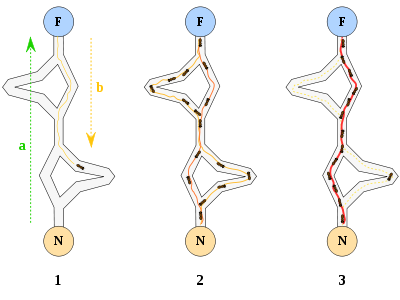
\includegraphics[width=5cm]{imagenes/feromona}
\end{figure}

\begin{figure}[h]
\caption{Ejemplo de uso de feromona}
\centering
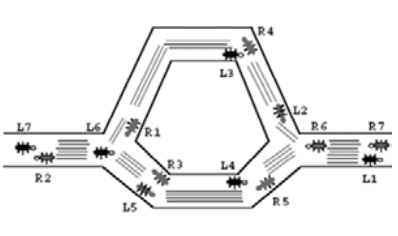
\includegraphics[width=5cm]{imagenes/feromona2}
\end{figure}

En la \textbf{figura 1} podemos ver una serie de iteraciones donde las hormigas llegan a la Fuente de comida y vuelven dejando feromonas y en la siguiente iteracion la solucion se ve influenciada por la feromona. Finalmente se lleva a una camino, el cual es elegido por casi todas las hormigas, siendo este la solucion final.

En la \textbf{figura 2} asumiendo que el nomero de lineas punteadas es proporcional a la cantidad de feromona, se puede ver como el camino inferior es más corto que el superior, muchas más hormigas transitarán por éste durante el mismo periodo de tiempo. Esto implica que en el camino más corto se acumula más feromona mucho más rápido. Después de cierto tiempo, la diferencia en la cantidad de feromona en los dos caminos es lo suficientemente grande para influenciar la decisión de las nuevas hormigas que entren a recorrer estas vías

Se puede ver que una gran ventaja de esta metaheuristica es que puede construir una solucion intercambiando informacion entre las distintas hormgias (soluciones), asi generar una solucion mejor de la que podrian generar individualmente.

Con el paso del tiempo el rastro de feromonas comienza a evaporarse, esto produce que los caminos pierdan su fuerza de atraccion, cuanto mas largo sea el camino, mas tiempo demorara una hormiga en recorrerlo, mas se evaporara la feromona y por ende seran menos frecuentado. Por su parte los caminos mas cortos (o mas optimos) tendran mayor cantidad de feromonas, por ende, mayor probabilidad de ser frecuentados.

ACO fue el primer algoritmo de optimizacion de Colonias de Hormigas desarrollado por Marco Dorigo en su tesis doctoral \cite{paperDorigo}. 

Algunas de las aplicaciones donde se utiliza esta metaheuristica:
\begin{enumerate}
\item El problema del viajante de comercion (TSP)
\item Optimización para el diseño de circuitos lógicos combinatorios
\item Problemas de enrutamiento de vehículos
\item Problema de la asignación de horarios
\item Aplicaciones a análisis de ADN y a procesos de producción
\item Partición de un grafo en árboles:
\item Otros
\end{enumerate}



\begin{thebibliography}{9}
\bibitem{wikipedia} 
https://en.wikipedia.org/wiki/Ant\_colony\_optimization\_algorithms

\bibitem{claseMetah} 
http://www-2.dc.uba.ar/materias/metah/meta2016-clase7.pdf

 
\bibitem{paperDorigo} 
http://people.idsia.ch/~gianni/Papers/CEC99.pdf

\bibitem{paperAplicaciones} 
Ant colony optimization: applications and trends. Carlos Algarin

\end{thebibliography}
\newpage
\section{El problema}\label{sec:problema}

Lorem ipsum dolor sit amet, consectetur adipisicing elit, sed do eiusmod
tempor incididunt ut labore et dolore magna aliqua. Ut enim ad minim veniam,
quis nostrud exercitation ullamco laboris nisi ut aliquip ex ea commodo
consequat. Duis aute irure dolor in reprehenderit in voluptate velit esse
cillum dolore eu fugiat nulla pariatur. Excepteur sint occaecat cupidatat non
proident, sunt in culpa qui officia deserunt mollit anim id est laborum.
\newpage
\section{Algoritmo Propuesto}\label{sec:algoritmo}
\subsection{Explicacion}

Lorem ipsum dolor sit amet, consectetur adipisicing elit, sed do eiusmod
tempor incididunt ut labore et dolore magna aliqua. Ut enim ad minim veniam,
quis nostrud exercitation ullamco laboris nisi ut aliquip ex ea commodo
consequat. Duis aute irure dolor in reprehenderit in voluptate velit esse
cillum dolore eu fugiat nulla pariatur. Excepteur sint occaecat cupidatat non
proident, sunt in culpa qui officia deserunt mollit anim id est laborum.

\subsection{Pseudocodigo}

\begin{codebox}
\Procname{$\proc{Insertion-Sort}(A)$}
\li \For $j \gets 2$ \To $\attrib{A}{length}$
\li \Do
$\id{key} \gets A[j]$
\li \Comment Insert $A[j]$ into the sorted sequence
$A[1 \twodots j-1]$.
\li $i \gets j-1$
\li \While $i > 0$ and $A[i] > \id{key}$
\li \Do
$A[i+1] \gets A[i]$
\li $i \gets i-1$
\End
\li $A[i+1] \gets \id{key}$
\End
\end{codebox}
\newpage
\section{Parametros}

En esta seccion se explicaran los parametros utilizados a la hora de hacer la experimentacion de todos los algoritmos. 

Notar que los algoritmos utilizados para comparar resultados son:

\begin{enumerate}
\item Scip (S)
\item Goloso (G)
\item Goloso Maximos Locales (GML)
\end{enumerate}

todos estos seran descriptos con mas detalles en la seccion \textbf{experimentacion}

Los parametros usados para estos algoritmos son:


\begin{enumerate}
\item Nx: Valor de la discretizacion del eje X.
\item Ny: Valor de la discretizacion del eje Y.
\item PMD: \textbf{Paso Mejora Discretizacion}, en el algoritmo GML se utiliza para \textbf{re-discretizar}, leer la explicacion en la seccion \textbf{experimentacion}
\item PMP: \textbf{Paso Movimiento Pad}, en el algoritmo GML se utiliza para el paso en que se mueven los Pads, a la hora de buscar el maximo local, leer la explicacion en la seccion \textbf{experimentacion}
\end{enumerate}

Por otro lado, para el algoritmo de colonia de hormgias se utilizaron los siguientes parametros:
							
\begin{enumerate}
\item IMPSR: \textbf{Intentos Meter Pad soluci\'on Random}, para ver cuando se termina de intentar meter pad en las soluciones tipo random (recordar que trabajamos en el continuo, y tenemos que decididr cuando ya creemos que se lleno la region).
\item CITF:  \textbf{Cantidad Intentos de Tapar una Feromona}, cantidad de pads que tapan a una feromona, para cada uno pruebo si es valido. Si ninguno es, se descarta esa feromona.
\item CSRI: \textbf{Cantidad soluciones Random Iniciales}, cantidad de soluciones de la primera iteracion. (soluciones random)
\item CI: \textbf{Cantidad Iteraciones}, cantidad iteraciones luego de la inicial.
\item CSNRPI: \textbf{Cantidad soluciones No Random Por Iteracion}, cantidad de soluciones por iteracion (Luego de la inicial).
\item MCBS: \textbf{Modo Chequeo Buena soluci\'on}, el modo para chequear cuando una soluci\'on es buena o mala (para enfriar o calentar la feromona, explicado mejor en la seccion \textbf{Algoritmo Propuesto}).
\item DF: \textbf{Discretizacion Feromona}, la discretizacion de la matrix de feromonas.
\item FCF: \textbf{Factor Cambio Feromona}, factor que se multiplica al actualizar la feromona (tambien se lo multiplica por el ogip normalizado)
\end{enumerate}













\newpage
\section{Experimentacion}\label{sec:experimentacion}

Lorem ipsum dolor sit amet, consectetur adipisicing elit, sed do eiusmod
tempor incididunt ut labore et dolore magna aliqua. Ut enim ad minim veniam,
quis nostrud exercitation ullamco laboris nisi ut aliquip ex ea commodo
consequat. Duis aute irure dolor in reprehenderit in voluptate velit esse
cillum dolore eu fugiat nulla pariatur. Excepteur sint occaecat cupidatat non
proident, sunt in culpa qui officia deserunt mollit anim id est laborum.
\newpage
\section{Resolucion alternativa}
La idea es usar un GRASP (Goloso Randomizado) y en general es encontrar el punto de la discretizacion donde el ogip valga mas y luego, dentro de un rango valido (un cuadrado) agarrar una lista de posibles pads, es decir, agregar a la lista todos los pads que pueden tapar a ese punto y luego agarrar un pad random para meter en la solucion y asi iterar sucesivamente. 

Una vez conseguida la solucion, hacer una busqueda local para tratar de mejorar la solucion. Y la forma de hacer la busqueda local es.

1- Para cada pad tratar de acercarlo a otro pads y al finalizar esto chequear si es posible meter otro nuevo pad.
2- Sacar algun pad con algun criterio y tratar de acomodar los pad restantes con algun algoritmo de programacion lineal entera.
3 -Otro
\newpage
\section{Programacion lineal entera}

En este trabajo se opt\'o por reducir el problema a un problema de conjunto independiente de peso m\'aximo en un grafo dado por la discretizaci\'on del \'area del yacimiento, que proporcion\'o buenos resultados en la pr\'actica. Dado un grafo $G=(V,E)$, un \textbf{conjunto independiente} es un conjunto $I\subseteq V$ de v\'ertices tal que $ij\not\in E$ para todo $i,j\in I$. Si adem\'as tenemos una funci\'on de peso W : V $\rightarrow \mathbb{R}$, el \textbf{peso} del conjunto independiente $I$ es $w(I) := \sum_{i\in I} w_i$. La motivaci\'on para este enfoque viene dada por el hecho de que el conjunto de pads de la soluci\'on conforma un conjunto de elementos no conflictivos entre s\'\i, situaci\'on que es modelada adecuadamente por medio de conjuntos independientes en un grafo. Sin embargo, esta reducci\'on trae aparejado un \emph{costo de discretizaci\'on}, que ser\'a mayor cuanto mayor sea el paso de discretizaci\'on seleccionado.

A grandes rasgos, el algoritmo propuesto est\'a compuesto por los siguientes puntos:
\begin{enumerate}
\item Discretizaci\'on $D\subseteq Y$ del \'area geogr\'afica del yacimiento.
\item Generaci\'on de un conjunto $T$ de pads posibles sobre la base de la discretizaci\'on $D$.
\item Planteo de un grafo $G=(T,E)$, de modo tal que cada conjunto independiente de $G$ corresponde a una soluci\'on factible del problema de optimizaci\'on del \'area de drenaje. Los v\'ertices del grafo reciben pesos adecuadamente definidos, de modo tal que el peso de cada conjunto independiente corresponde a la funci\'on objetivo de la soluci\'on factible.
\item B\'usqueda de un conjunto independiente de peso m\'aximo sobre $G$ por medio de un modelo de programaci\'on lineal entera, para obtener una soluci\'on $P$ al problema.
\end{enumerate}
Describimos a continuaci\'on cada punto del algoritmo. Para esto, sean $\Delta_x$, $\Delta_y$ $\in$ $\mathbb{R}_{+}$ los \textbf{pasos de discretizaci\'on} y sea $A=\{\alpha_1,\dots,\alpha_p\}$ un conjunto de \'angulos posibles, de modo tal que $\alpha_i\in[\alpha-\beta,\alpha+\beta]$ para $i=1,\dots,p$. En nuestra implementaci\'on computacional, tomamos $A=\{\alpha-\beta,\alpha,\alpha+\beta\}$.


\noindent\textbf{Discretizaci\'on.} El primer paso del algoritmo consiste en generar una discretizaci\'on $D=\{(x_i,y_i)\}_{i=1}^m$ por filas y columnas del \'area del yacimiento, de modo tal que dos puntos consecutivos de una misma fila est\'en a distancia $\Delta_x$ y dos puntos consecutivos de una misma columna est\'en a distancia $\Delta_y$. Para esto, se genera un reticulado de puntos en el plano con \'angulo $\alpha$.


\noindent\textbf{Generaci\'on de pads.} Para cada punto $(x,y)\in D$ de la discretizaci\'on, cada configuraci\'on $S\in\S$ y cada \'angulo $i\in\{1,\dots,p\}$, se incluye en el conjunto $T$ un pad $P$ con configuraci\'on $S$, centrado en $(x,y)$ y rotado en \'angulo $\alpha_i$, siempre que el pad $P$ (i) est\'e incluido completamente dentro de $Y$ y (ii) su locaci\'on $L$ no interseque con ning\'un obst\'aculo. Para determinar este \'ultimo punto, se consideran como centros posibles de la locaci\'on el punto $(x,y)$ y ocho puntos equiangulados sobre la circunferencia de centro $(x,y)$ y radio $tol_S$, y se considera que se cumple la condici\'on (ii) si para alguno de estos puntos, la locaci\'on centrada en ese punto no interseca a ning\'un obst\'aculo. Este enfoque es arbitrario e incurre en un nuevo error de discretizaci\'on, pero se observ\'o que genera resultados aceptables en la pr\'actica.


\noindent\textbf{Grafo de conflictos.} Se genera un grafo $G=(T,E)$ cuyos v\'ertices est\'an dados por todos los pads generados en el punto anterior, y cuyas aristas unen pares de pads con intersecci\'on no vac\'\i a. El conjunto $E$ est\'a compuesto por los pares $(P_1,P_2)$ tales que existe alg\'un punto $(x,y)\in D$ con $(x,y)\in P_1$ y $(x,y)\in P_2$. Esta definici\'on de $E$ permite que existan pares de pads con peque\~nas superposiciones pero sin una arista que los una en $G$. Esto sucede cuando la intersecci\'on no contiene ning\'un punto de la discretizaci\'on $D$, lo cual puede ocurrir s\'olo cuando la superposici\'on es peque\~na. De este modo, se maneja adecuadamente la restricci\'on el\'astica de no superposici\'on de pads.

\noindent\textbf{Obtenci\'on de una soluci\'on.} Se plantea y se resuelve la siguiente formulaci\'on de conjunto independiente con peso m\'aximo sobre $G$, usando las restricciones clique sobre todos los puntos de la discretizaci\'on. En este modelo, se tiene una variable binaria $x_P$ por cada pad, de modo tal que $x_P=1$ si y s\'olo si el pad $P$ se incluye en la soluci\'on.


\begin{center}
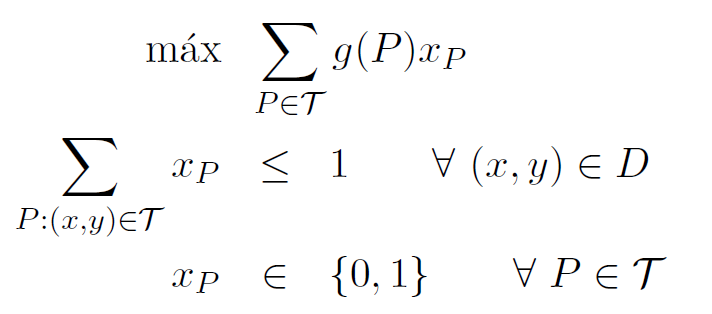
\includegraphics[width=0.5\textwidth]{imagenes/formula}
\end{center}




El coeficiente $g(P)$ asociado con la variable $x_P$ en la funci\'on objetivo es $g(P) = neto(P)$ si se optimiza el beneficio total (dado por la venta de la producci\'on total esperada menos los costos de construcci\'on), o bien $g(P) = area(P)$ si se optimiza el \'area total cubierta. 
Dado que los puntos de la discretizaci\'on $D$ generan todas las cliques maximales de $G$ (aunque no todo punto de $D$ genera necesariamente una clique maximal), esta formulaci\'on incluye todas las restricciones de la formulaci\'on por cliques del problema de conjunto independiente de peso m\'aximo, y se espera que sea m\'as fuerte que una formulaci\'on con una restricci\'on por arista. Dadas las caracter\'\i sticas aproximadas del procedimiento, no resulta imprescindible en la pr\'actica resolver en forma \'optima el modelo de programaci\'on entera planteado, aunque la pr\'oxima secci\'on muestra que en general este modelo se resuelve en forma exacta para tama\~nos de instancia razonables.

La generaci\'on de la discretizaci\'on $D$ es un paso clave dentro del algoritmo. Si los pasos de discretizaci\'on $\Delta_x$ y $\Delta_y$ son demasiado grandes, entonces no se generar\'a un n\'umero suficientemente grande y variado de pads en $T$ y la soluci\'on ser\'a de peor calidad, adem\'as de incluir potencialmente superposiciones entre los pads seleccionados, dado el modo en el que se generan las aristas de $G$. Sin embargo, a medida que $\Delta_x$ y $\Delta_y$ disminuyen se espera que estos efectos se vean minimizados, y que caigan por debajo de los errores de mediciones y de los par\'ametros de seguridad habituales en la industria hidrocarbur\'\i fera. A medida que  tienden a cero, la soluci\'on generada por este procedimiento tiende a la soluci\'on \'optima. Los experimentos computacionales presentados en la pr\'oxima secci\'on muestran que eligiendo adecuadamente los valores de $\Delta_x$ y $\Delta_y$ se obtienen buenos resultados.

\newpage
\section{Conclusion}\label{sec:conclusion}

Lorem ipsum dolor sit amet, consectetur adipisicing elit, sed do eiusmod
tempor incididunt ut labore et dolore magna aliqua. Ut enim ad minim veniam,
quis nostrud exercitation ullamco laboris nisi ut aliquip ex ea commodo
consequat. Duis aute irure dolor in reprehenderit in voluptate velit esse
cillum dolore eu fugiat nulla pariatur. Excepteur sint occaecat cupidatat non
proident, sunt in culpa qui officia deserunt mollit anim id est laborum.
\newpage
\section{Anexo}

En la presente seccion se muestran \text{todos} los experimentos realizados con distintas instancias, variando el tamanio de la region, de las semillas, de las toleraciones, la cantidad de semillas, angulos, restrinciones, etc.
Para cada subsection se cuenta con 5 graficos, el primero correspondiente a los resultados obtenidos con la tecnica de \text{Programacion lineal entera}, el segundo utilizadno un algortimo \textbf{Goloso},el tercero utilizadno el algortimo llamado \textbf{Goloso Maximos Locales}, el cuarto para el algoritmo utilizando \textbf{Colonia de Hormigas} y el quinto utilizando \textbf{Colonia de Hormiga Version 2}. 

Para mas informacion sobre los algoritmos ver la seccion \text{Experimentacion} y para mas informacion sobre las tablas ver la seccion \textbf{Parametros}.
\subsection{0G100x100\_muchos}

\begin{center}
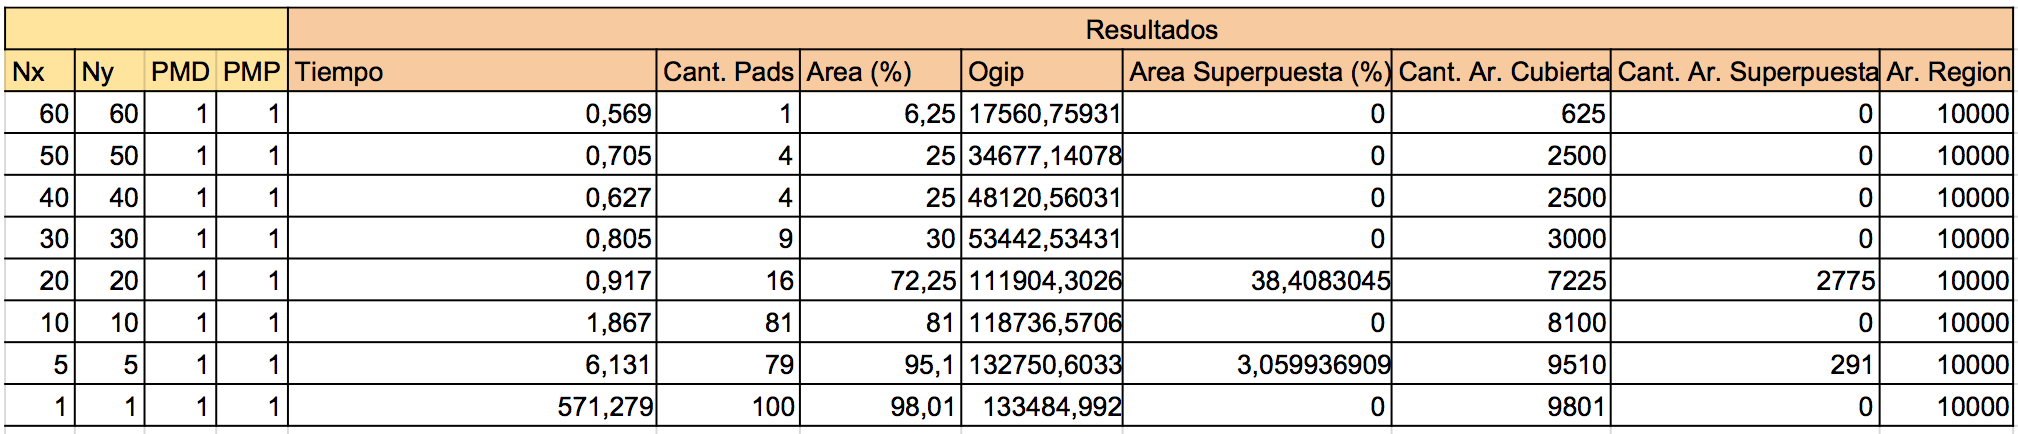
\includegraphics[width=1\textwidth]{imagenes/S_0G100x100_muchos}
\end{center}

\begin{center}
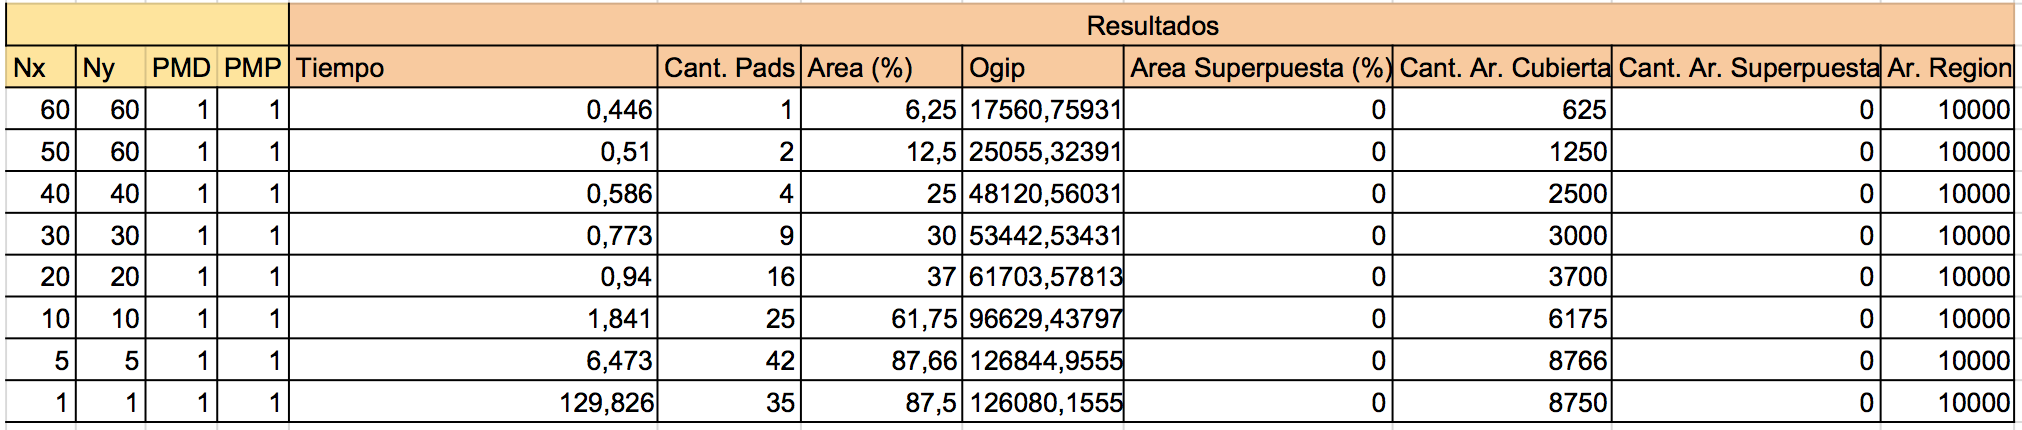
\includegraphics[width=1\textwidth]{imagenes/G_0G100x100_muchos}
\end{center}

\begin{center}
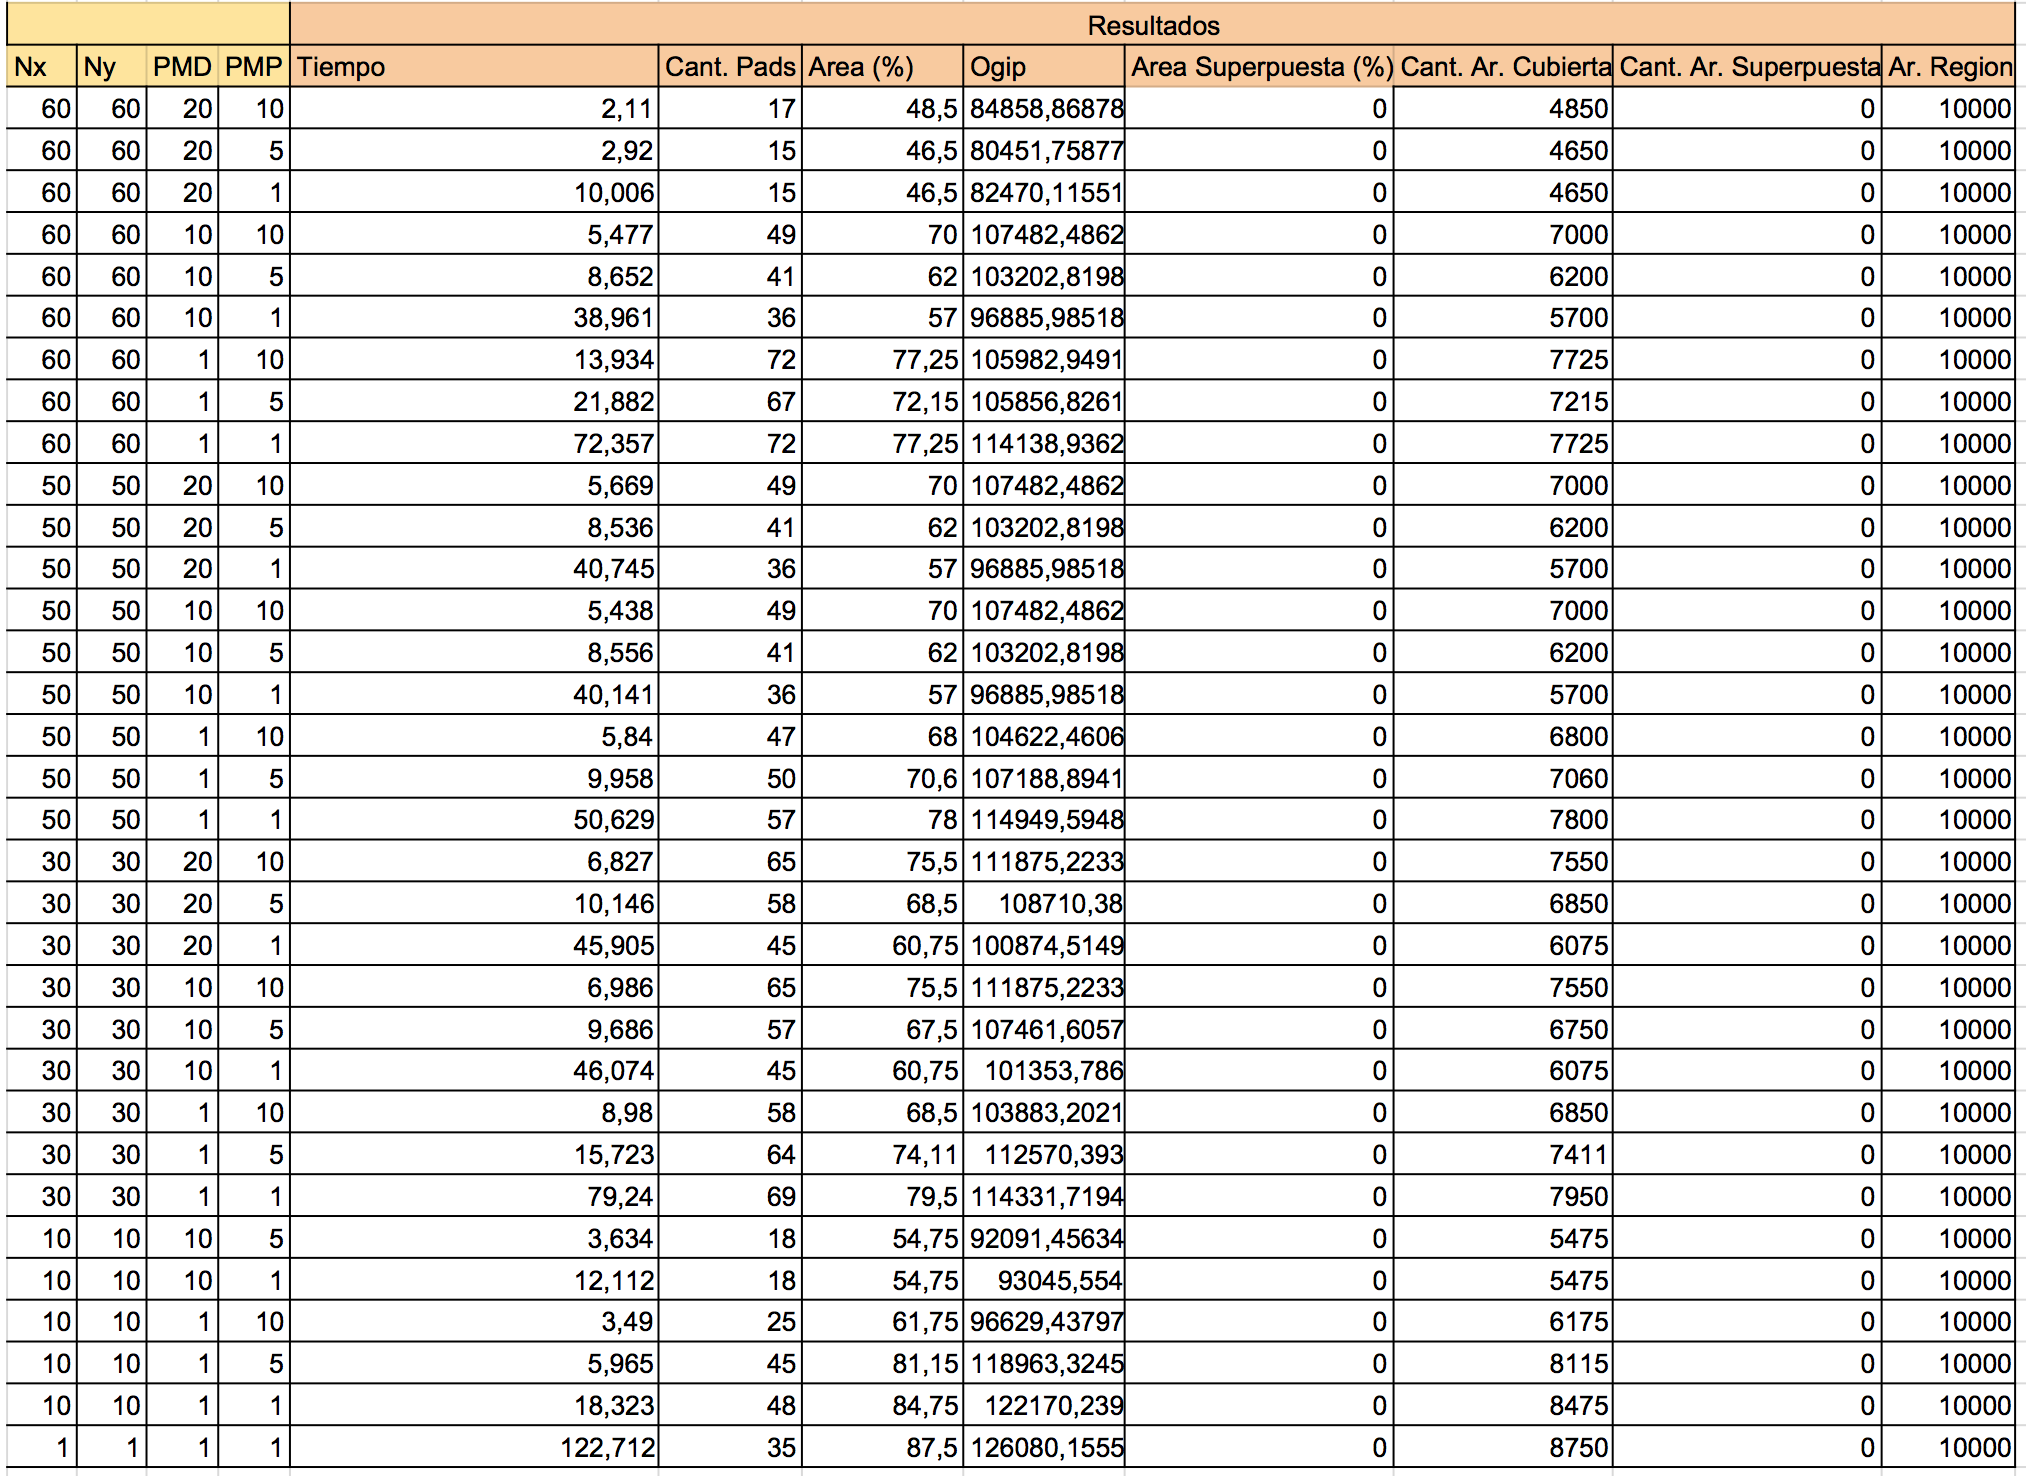
\includegraphics[width=0.9\textwidth]{imagenes/GML_0G100x100_muchos}
\end{center}

\begin{center}
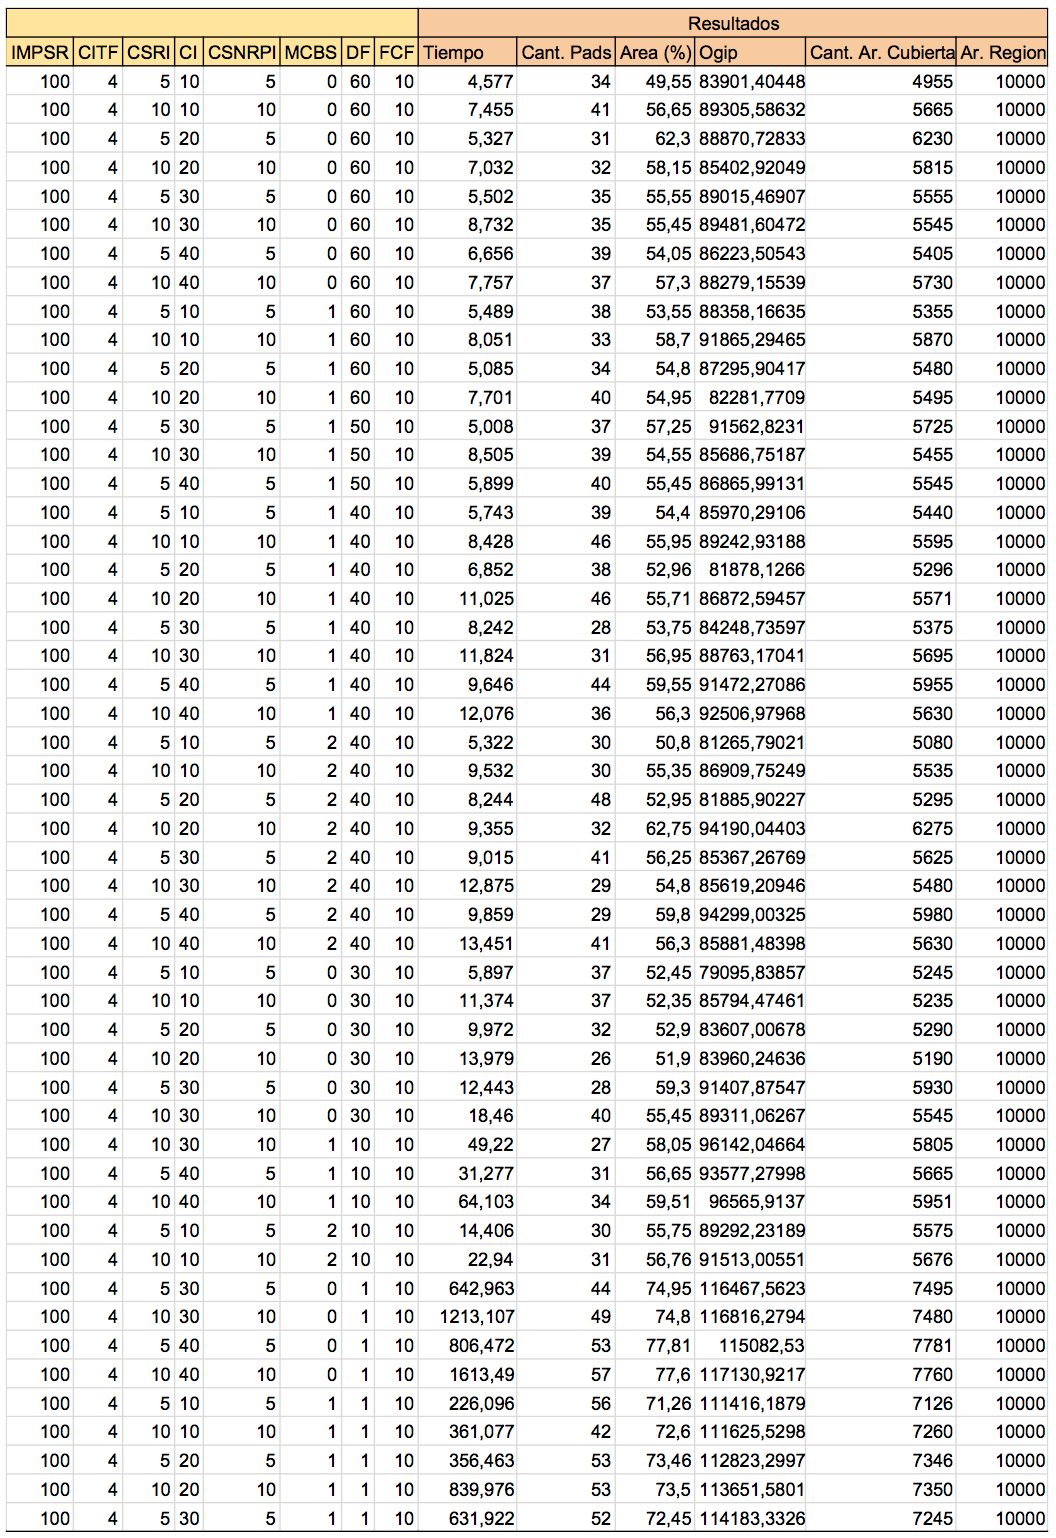
\includegraphics[width=1\textwidth]{imagenes/0G100x100_muchos_V1}
\end{center}

\begin{center}
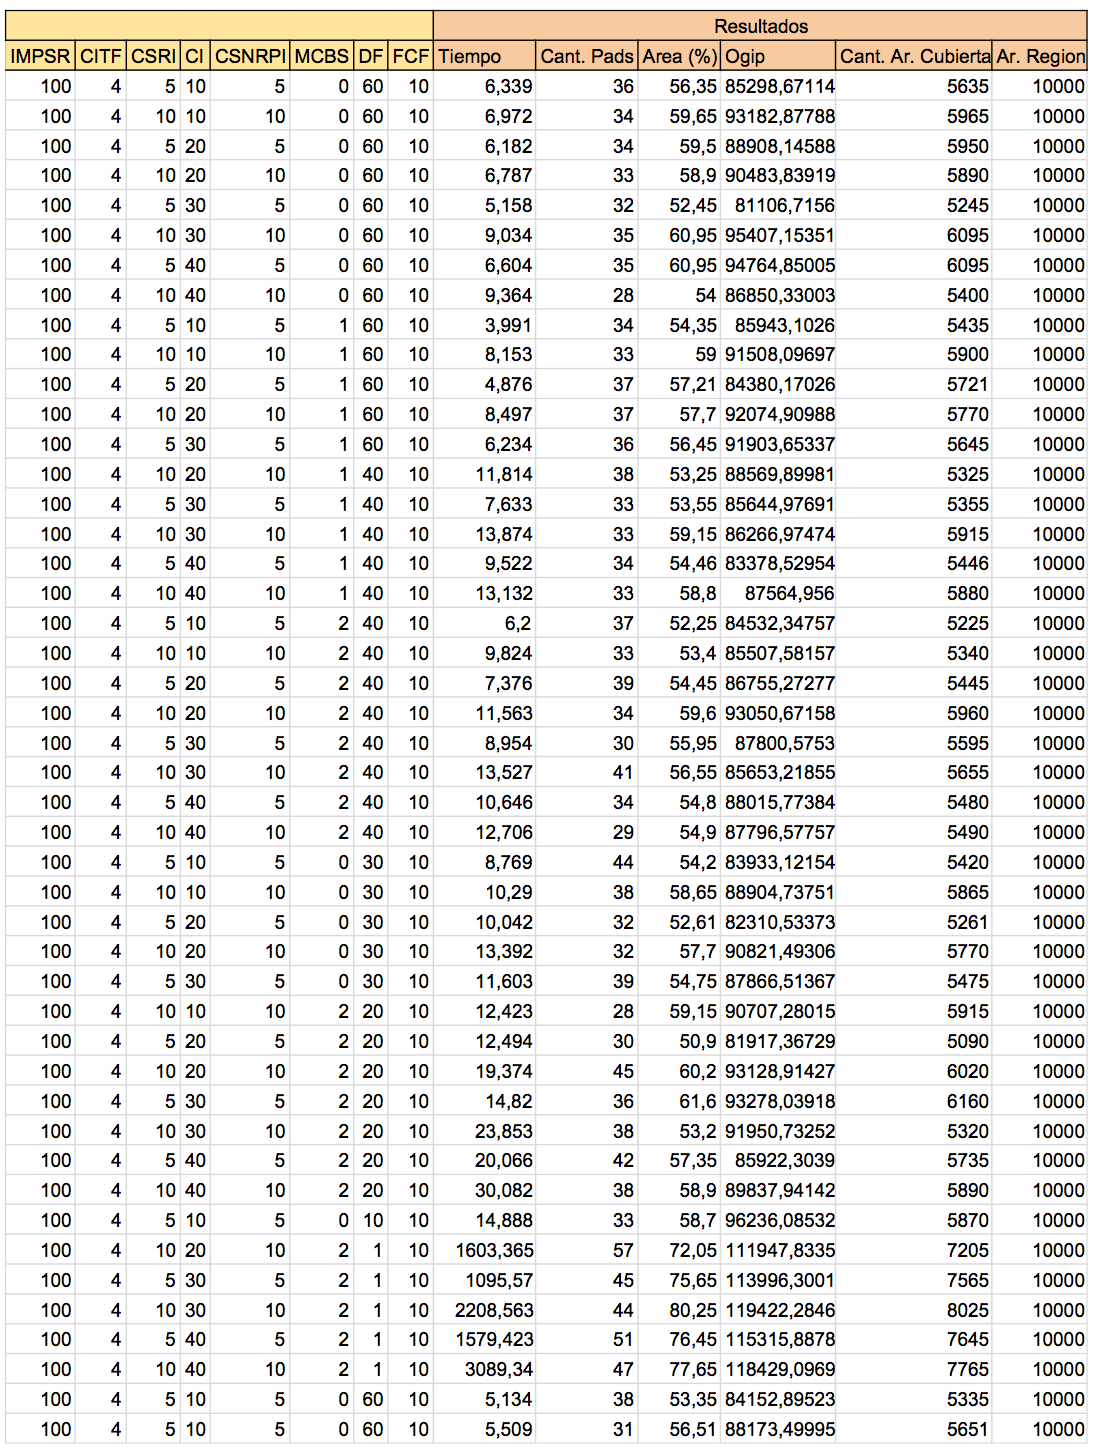
\includegraphics[width=1\textwidth]{imagenes/0G100x100_muchos_V2}
\end{center}

\subsection{0G100x100\_pocos}

\begin{center}
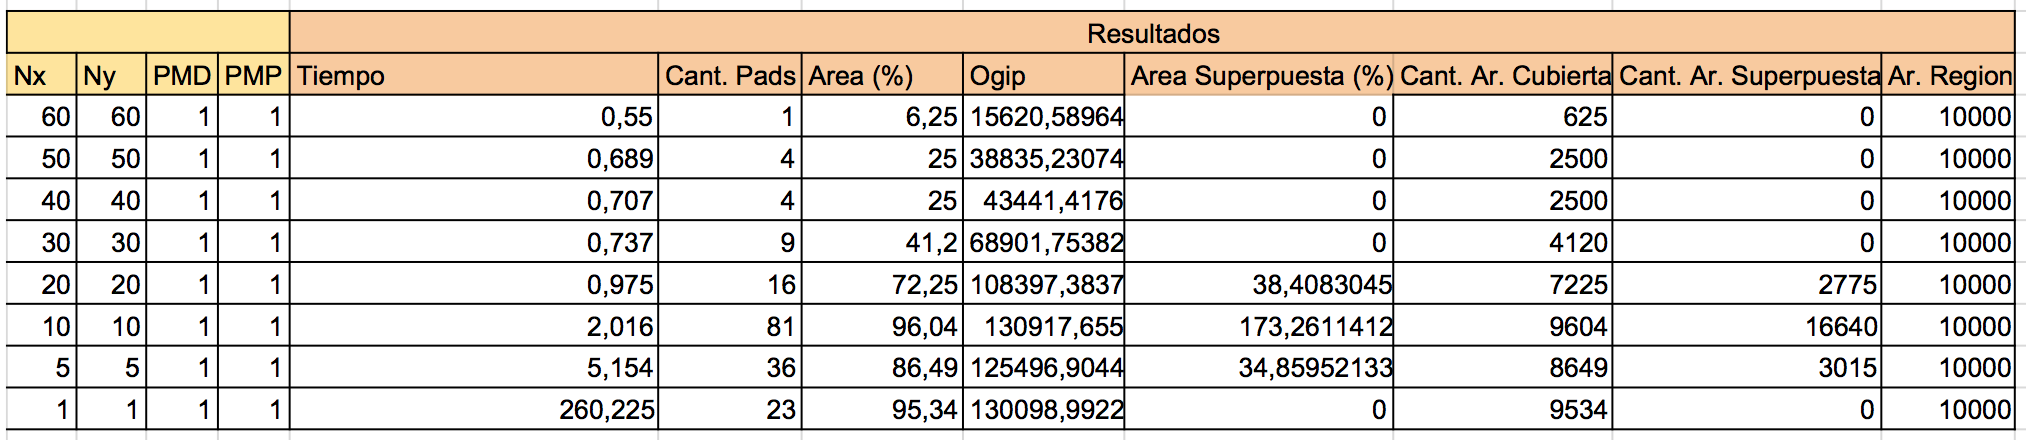
\includegraphics[width=1\textwidth]{imagenes/S_0G100x100_pocos}
\end{center}

\begin{center}
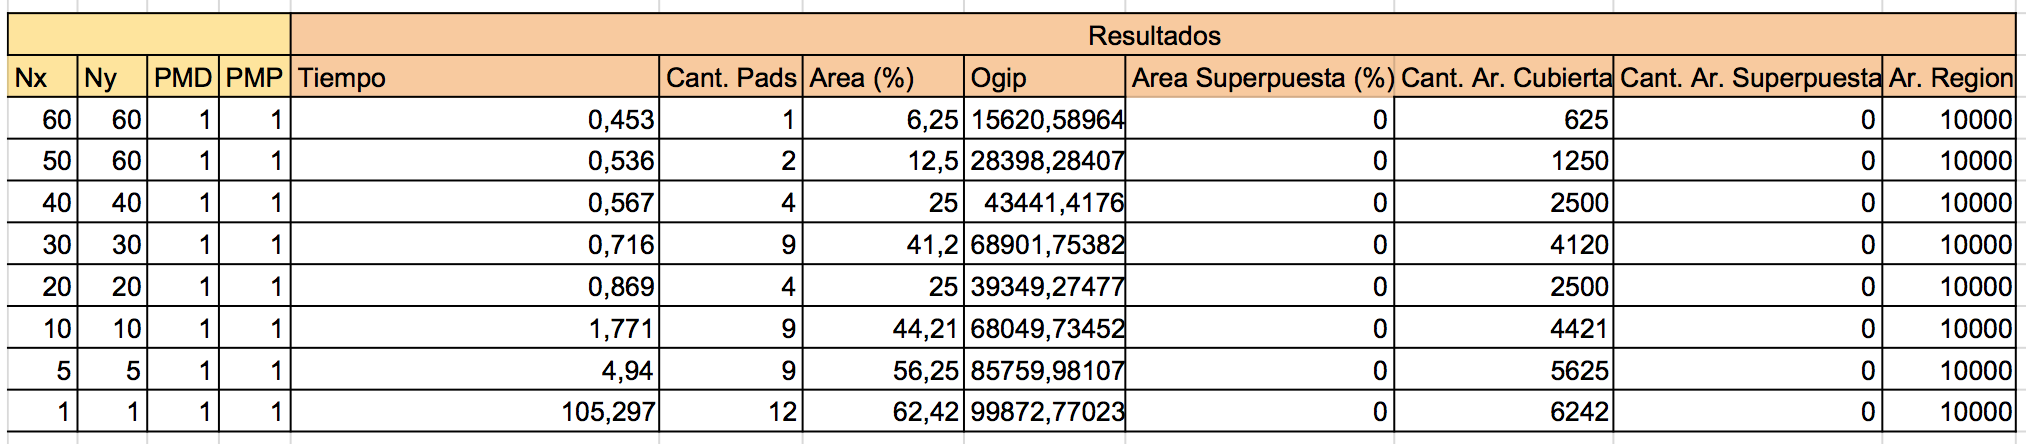
\includegraphics[width=1\textwidth]{imagenes/G_0G100x100_pocos}
\end{center}

\begin{center}
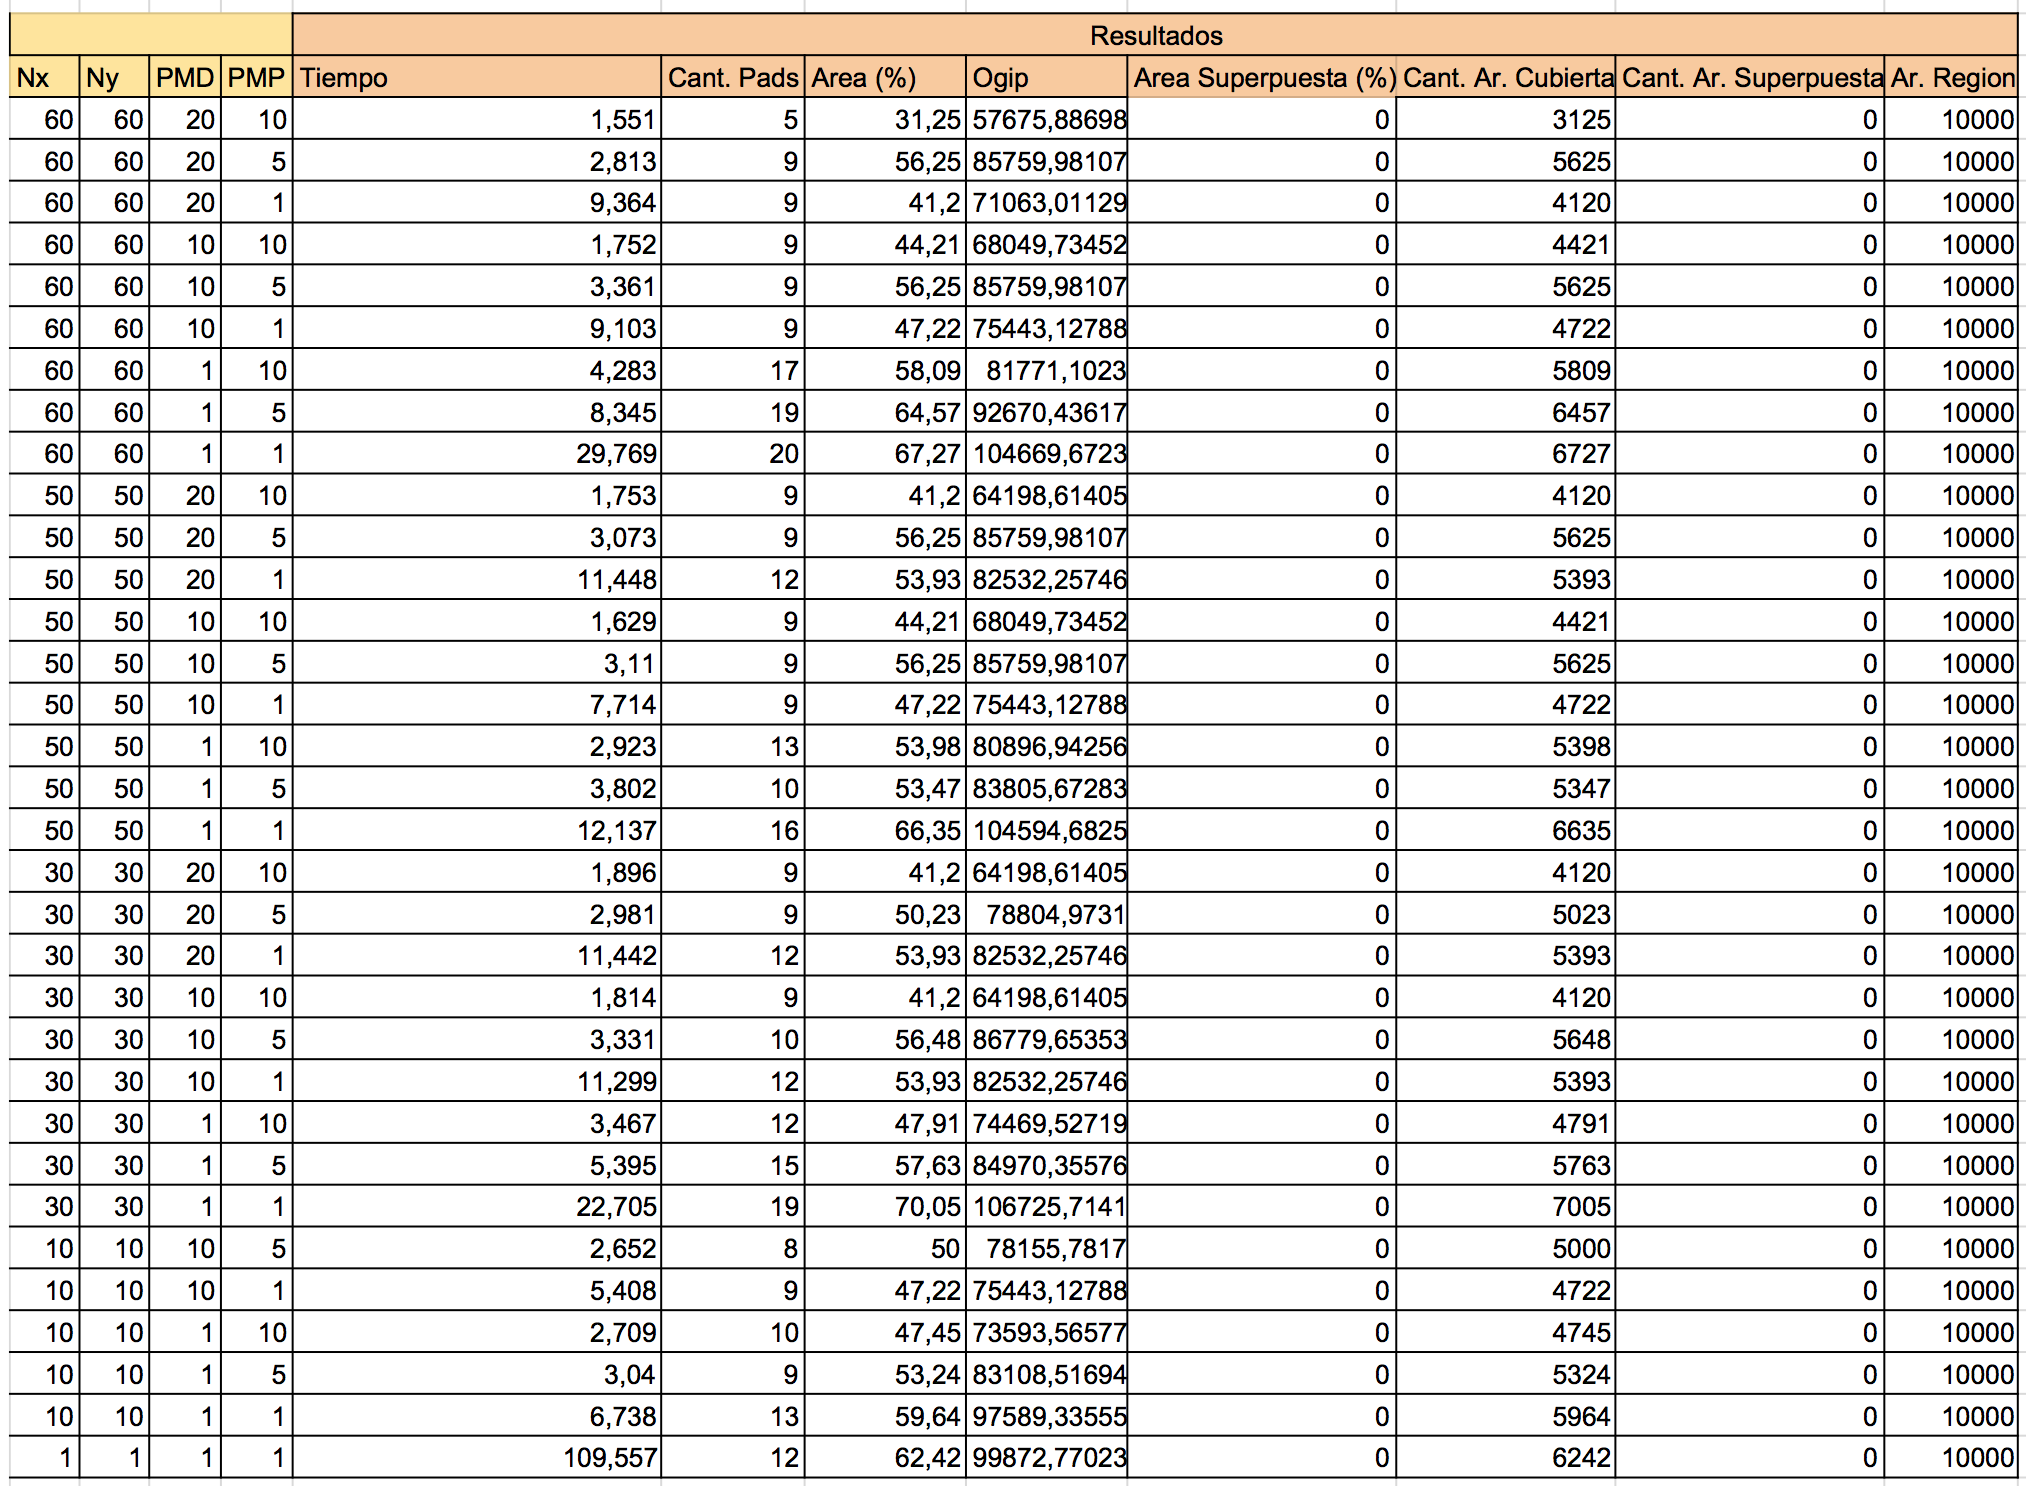
\includegraphics[width=1\textwidth]{imagenes/GML_0G100x100_pocos}
\end{center}

\begin{center}
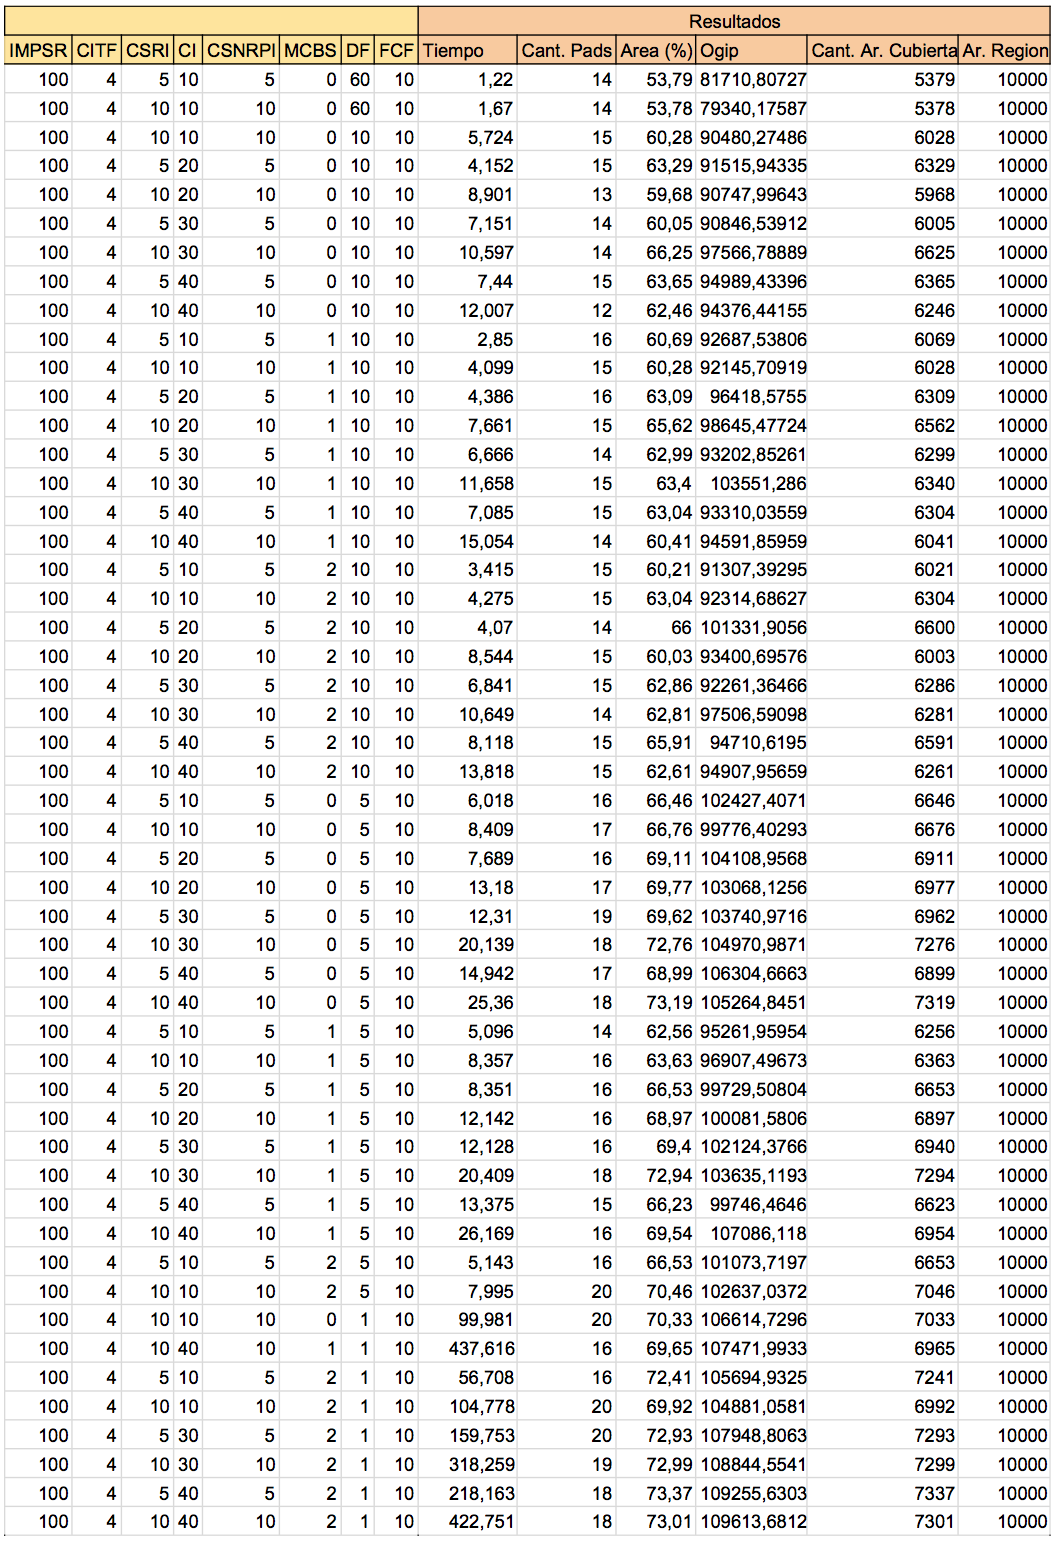
\includegraphics[width=1\textwidth]{imagenes/0G100x100_pocos_V1}
\end{center}

\begin{center}
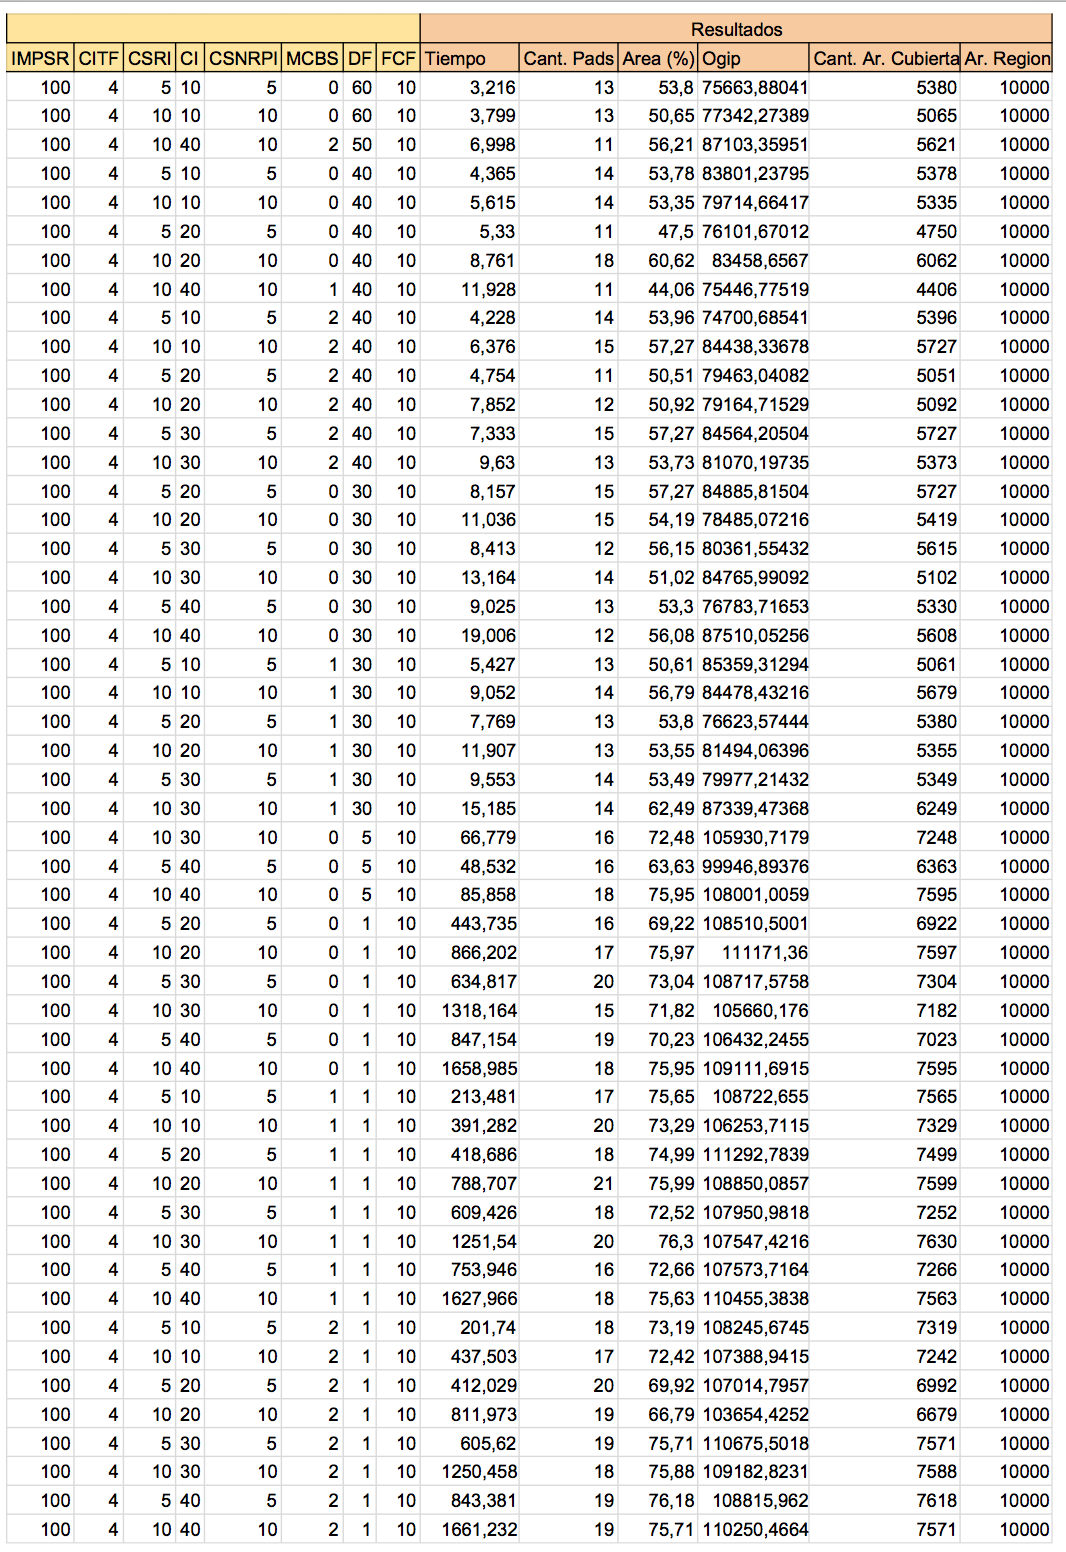
\includegraphics[width=1\textwidth]{imagenes/0G100x100_pocos_V2}
\end{center}

\subsection{45G100x100\_pocos}

\begin{center}
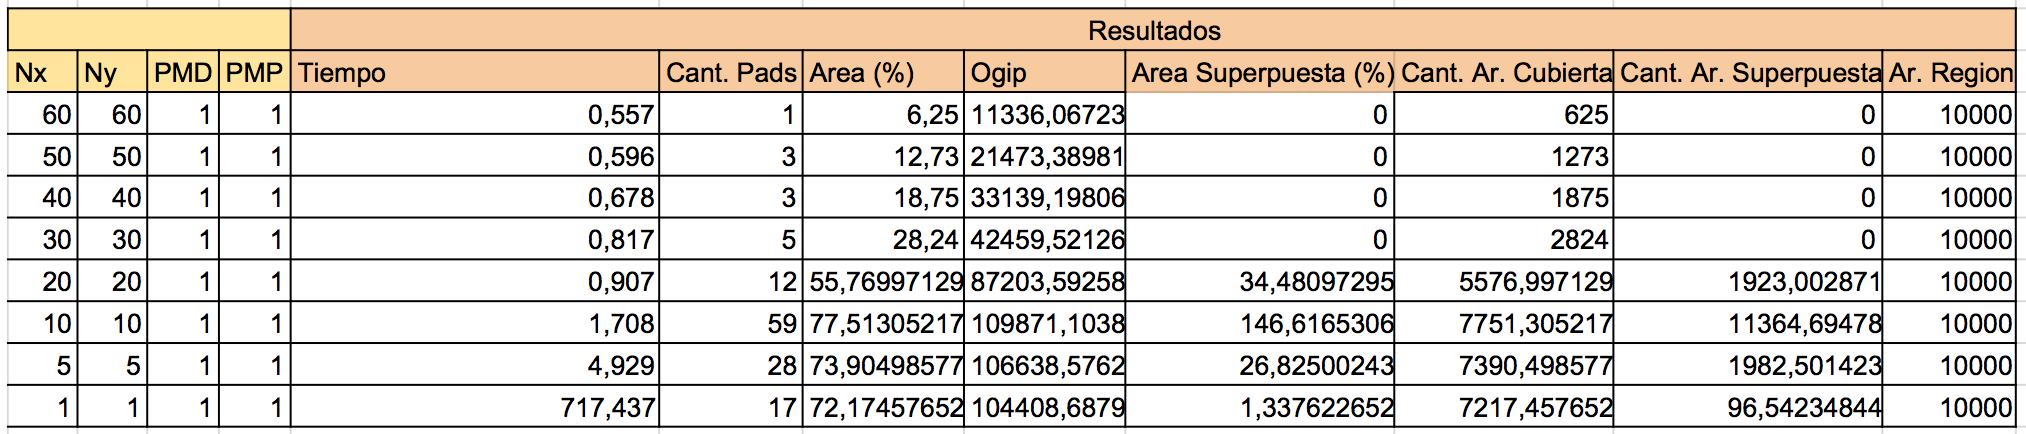
\includegraphics[width=1\textwidth]{imagenes/S_45G100x100_pocos}
\end{center}

\begin{center}
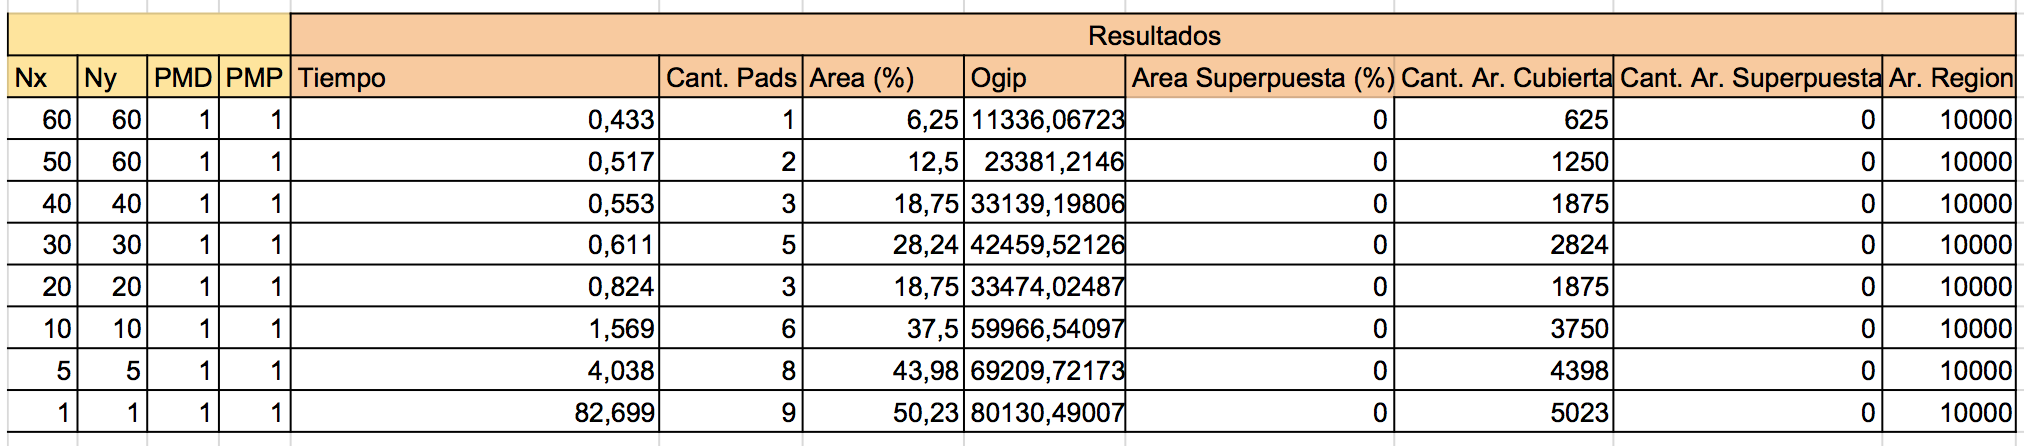
\includegraphics[width=1\textwidth]{imagenes/G_45G100x100_pocos}
\end{center}

\begin{center}
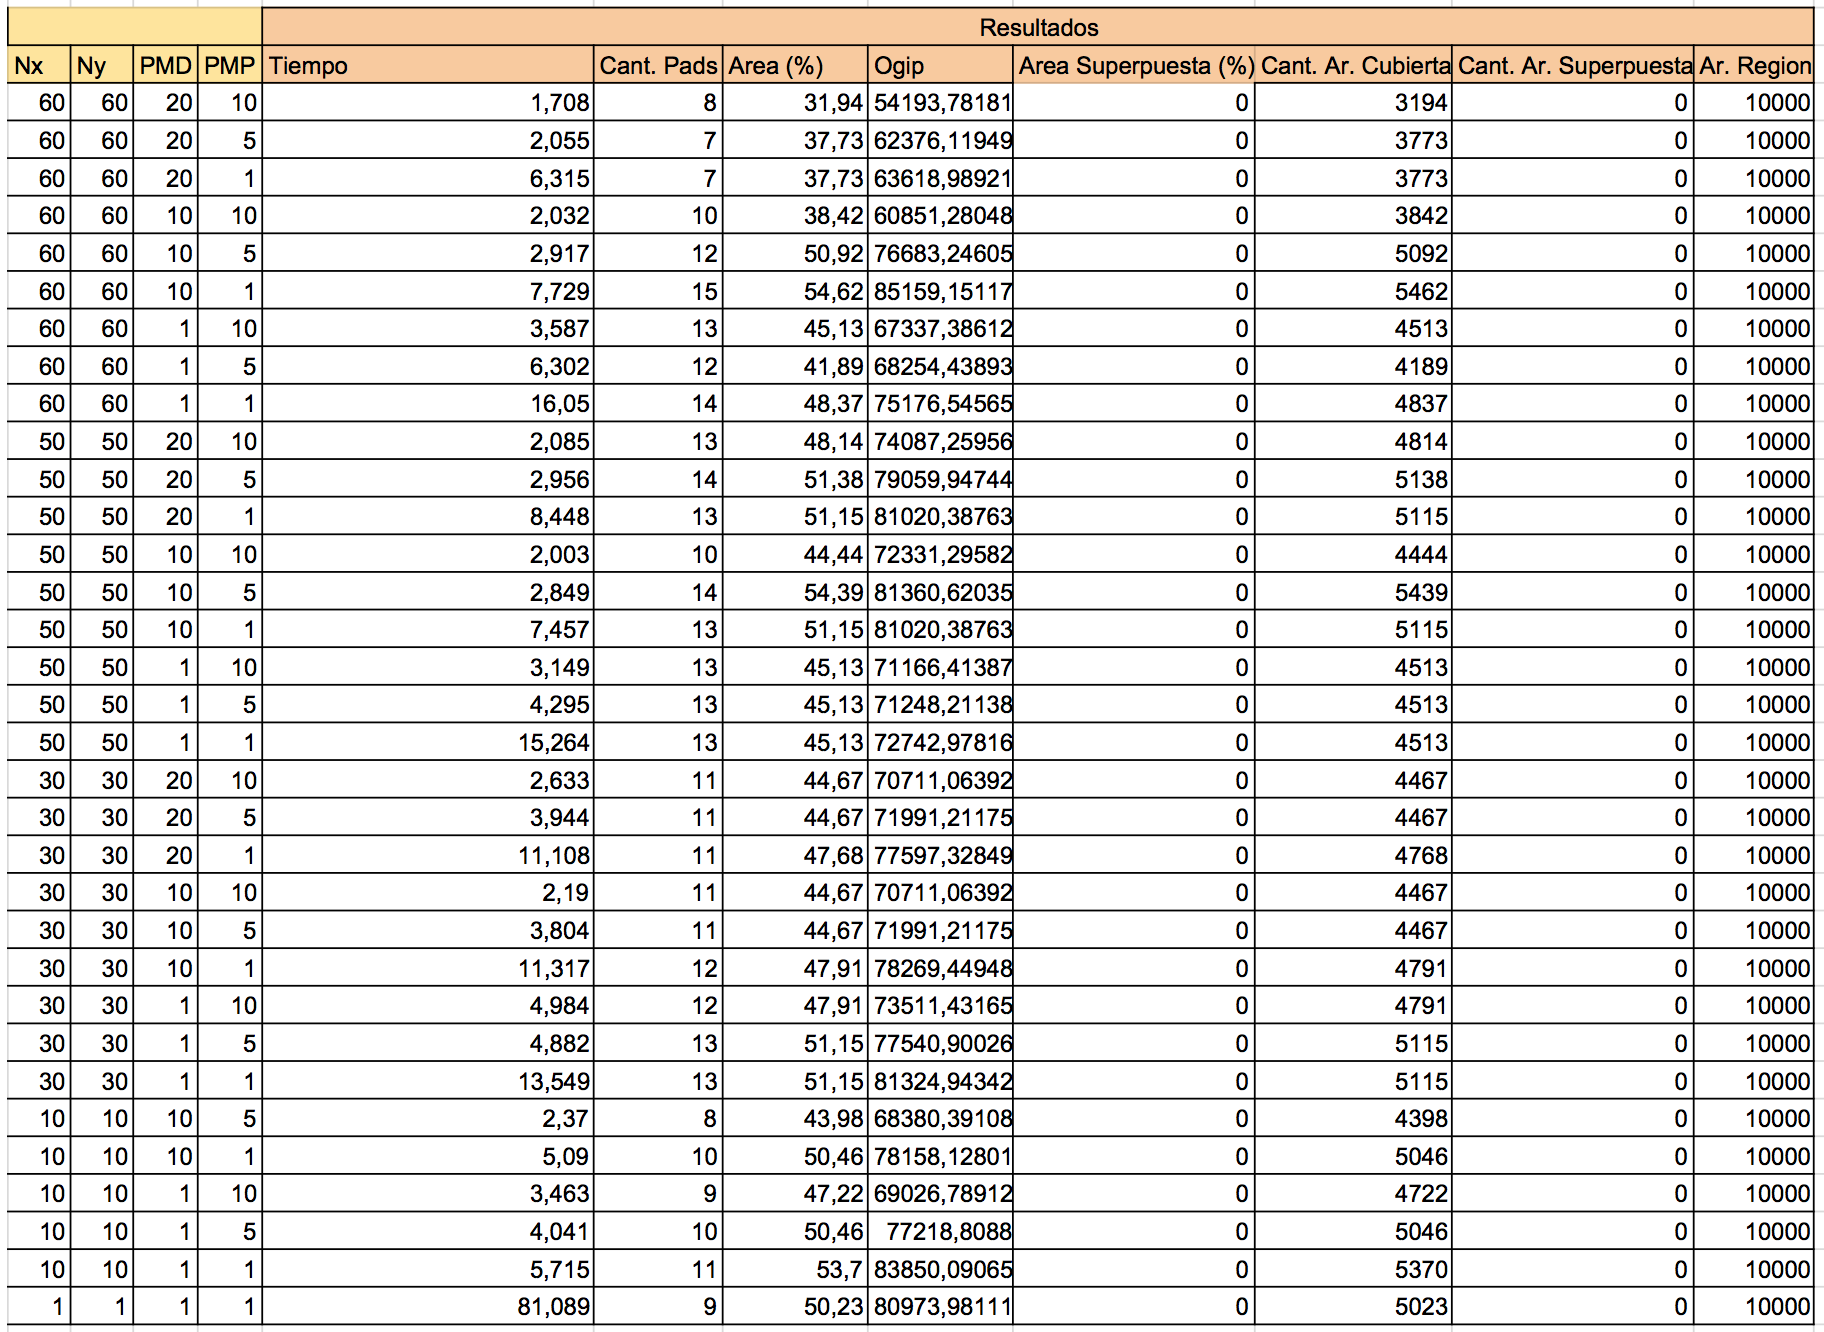
\includegraphics[width=1\textwidth]{imagenes/GML_45G100x100_pocos}
\end{center}

\begin{center}
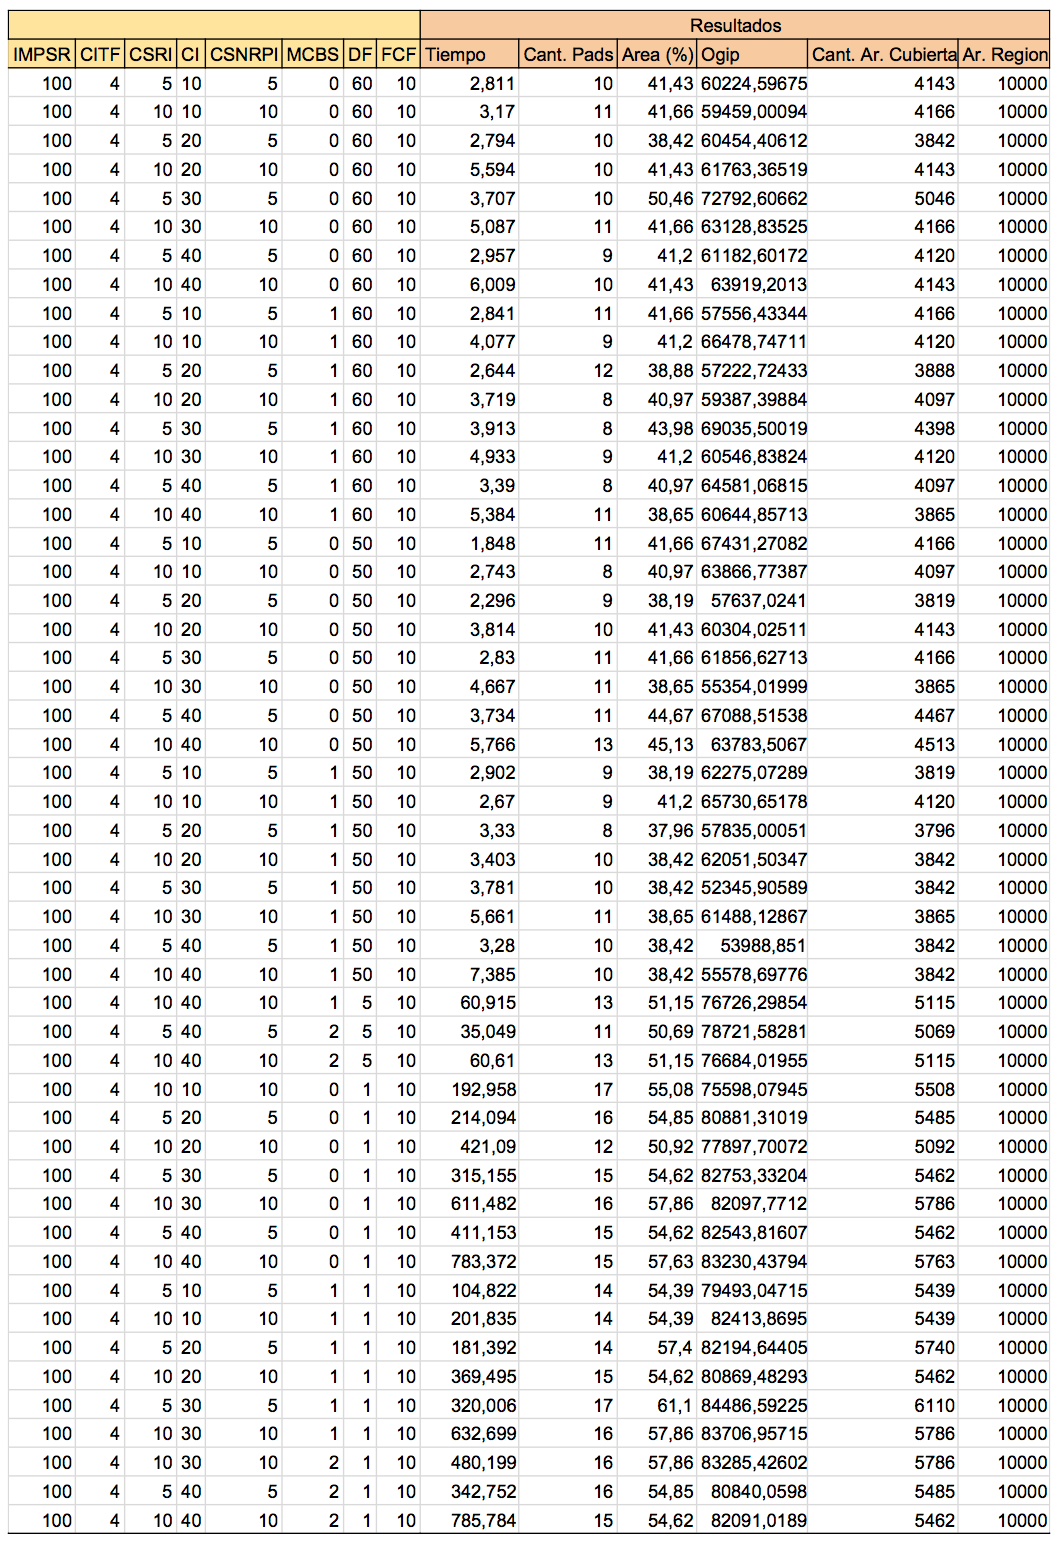
\includegraphics[width=1\textwidth]{imagenes/45G100x100_pocos_V1}
\end{center}

\begin{center}
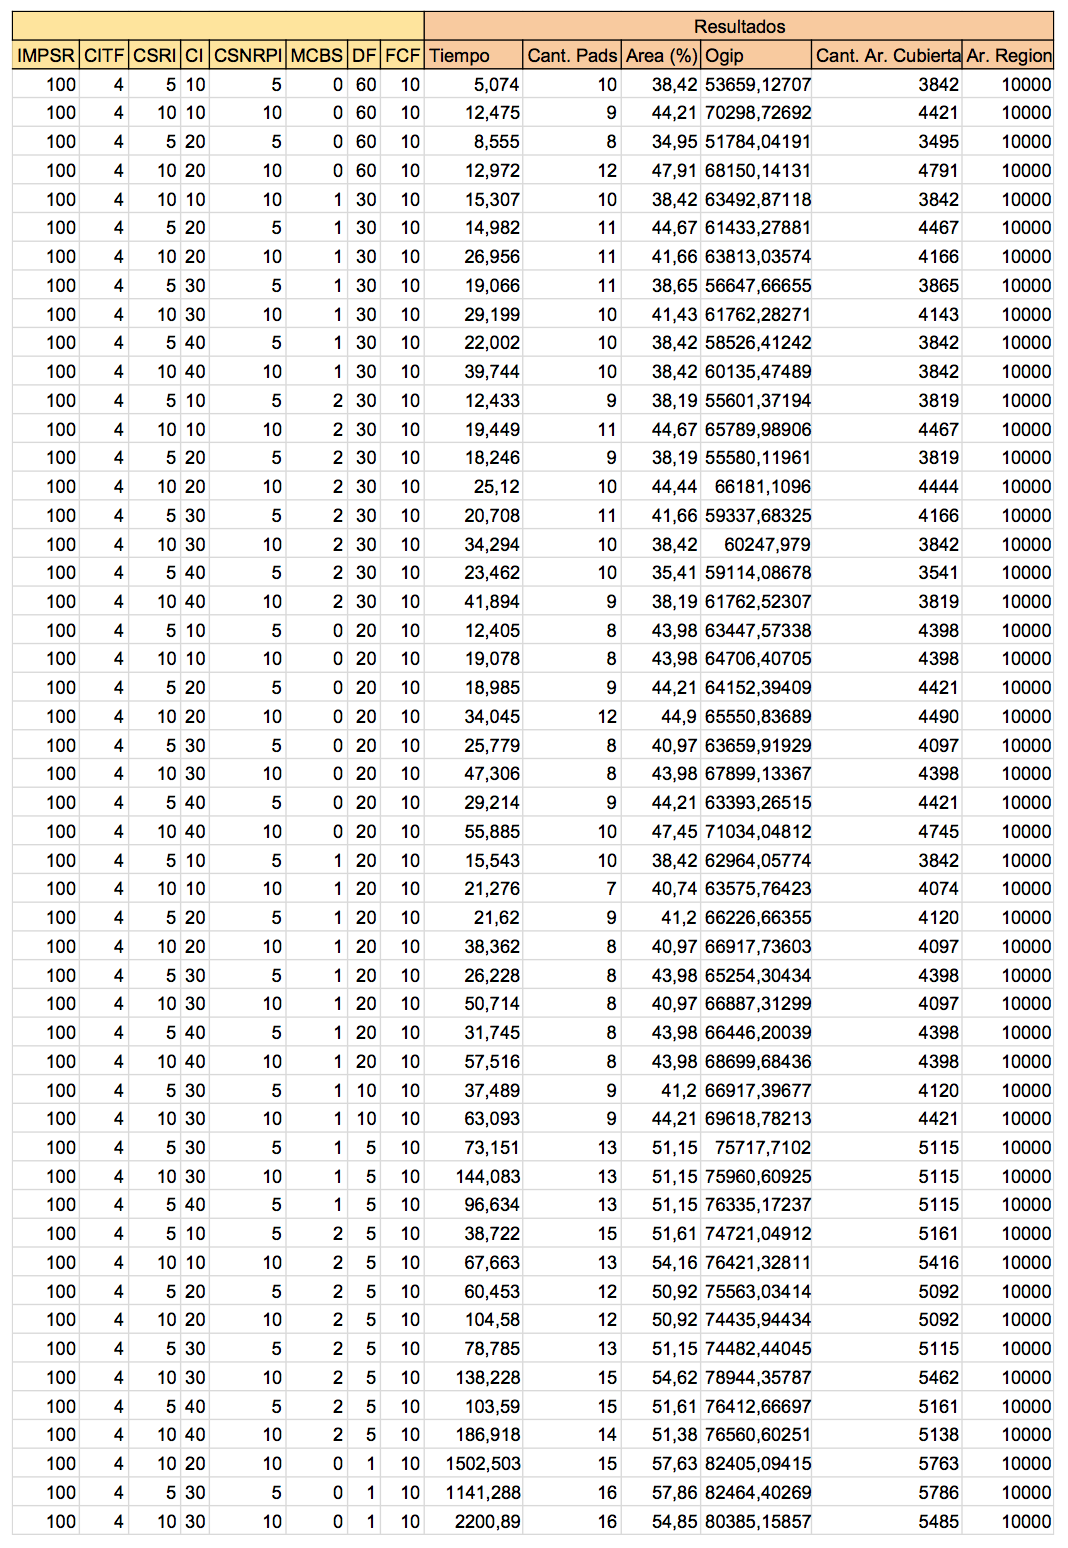
\includegraphics[width=1\textwidth]{imagenes/45G100x100_pocos_V2}
\end{center}

\subsection{45G100x100\_muchos}

\begin{center}
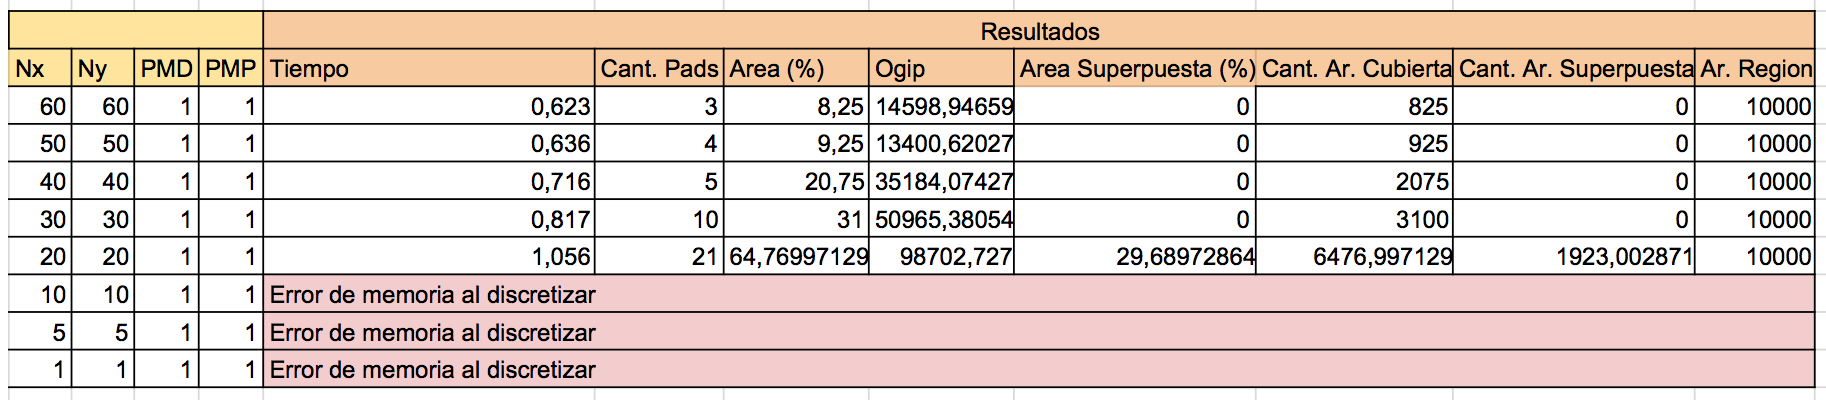
\includegraphics[width=1\textwidth]{imagenes/S_45G100x100_muchos}
\end{center}

\begin{center}
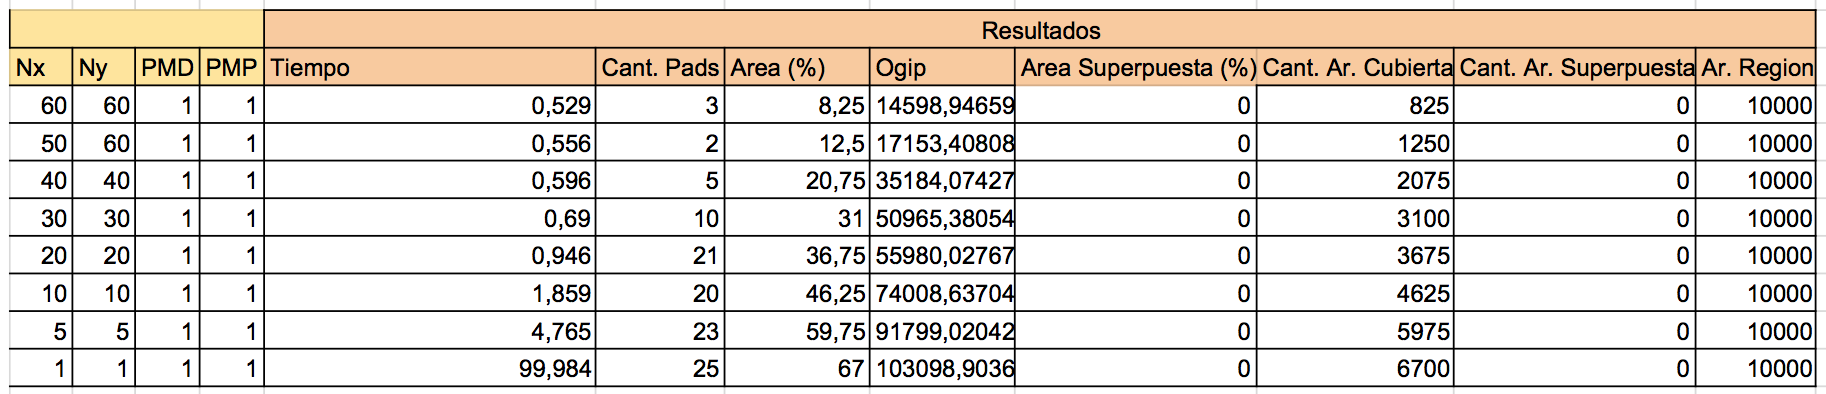
\includegraphics[width=1\textwidth]{imagenes/G_45G100x100_muchos}
\end{center}

\begin{center}
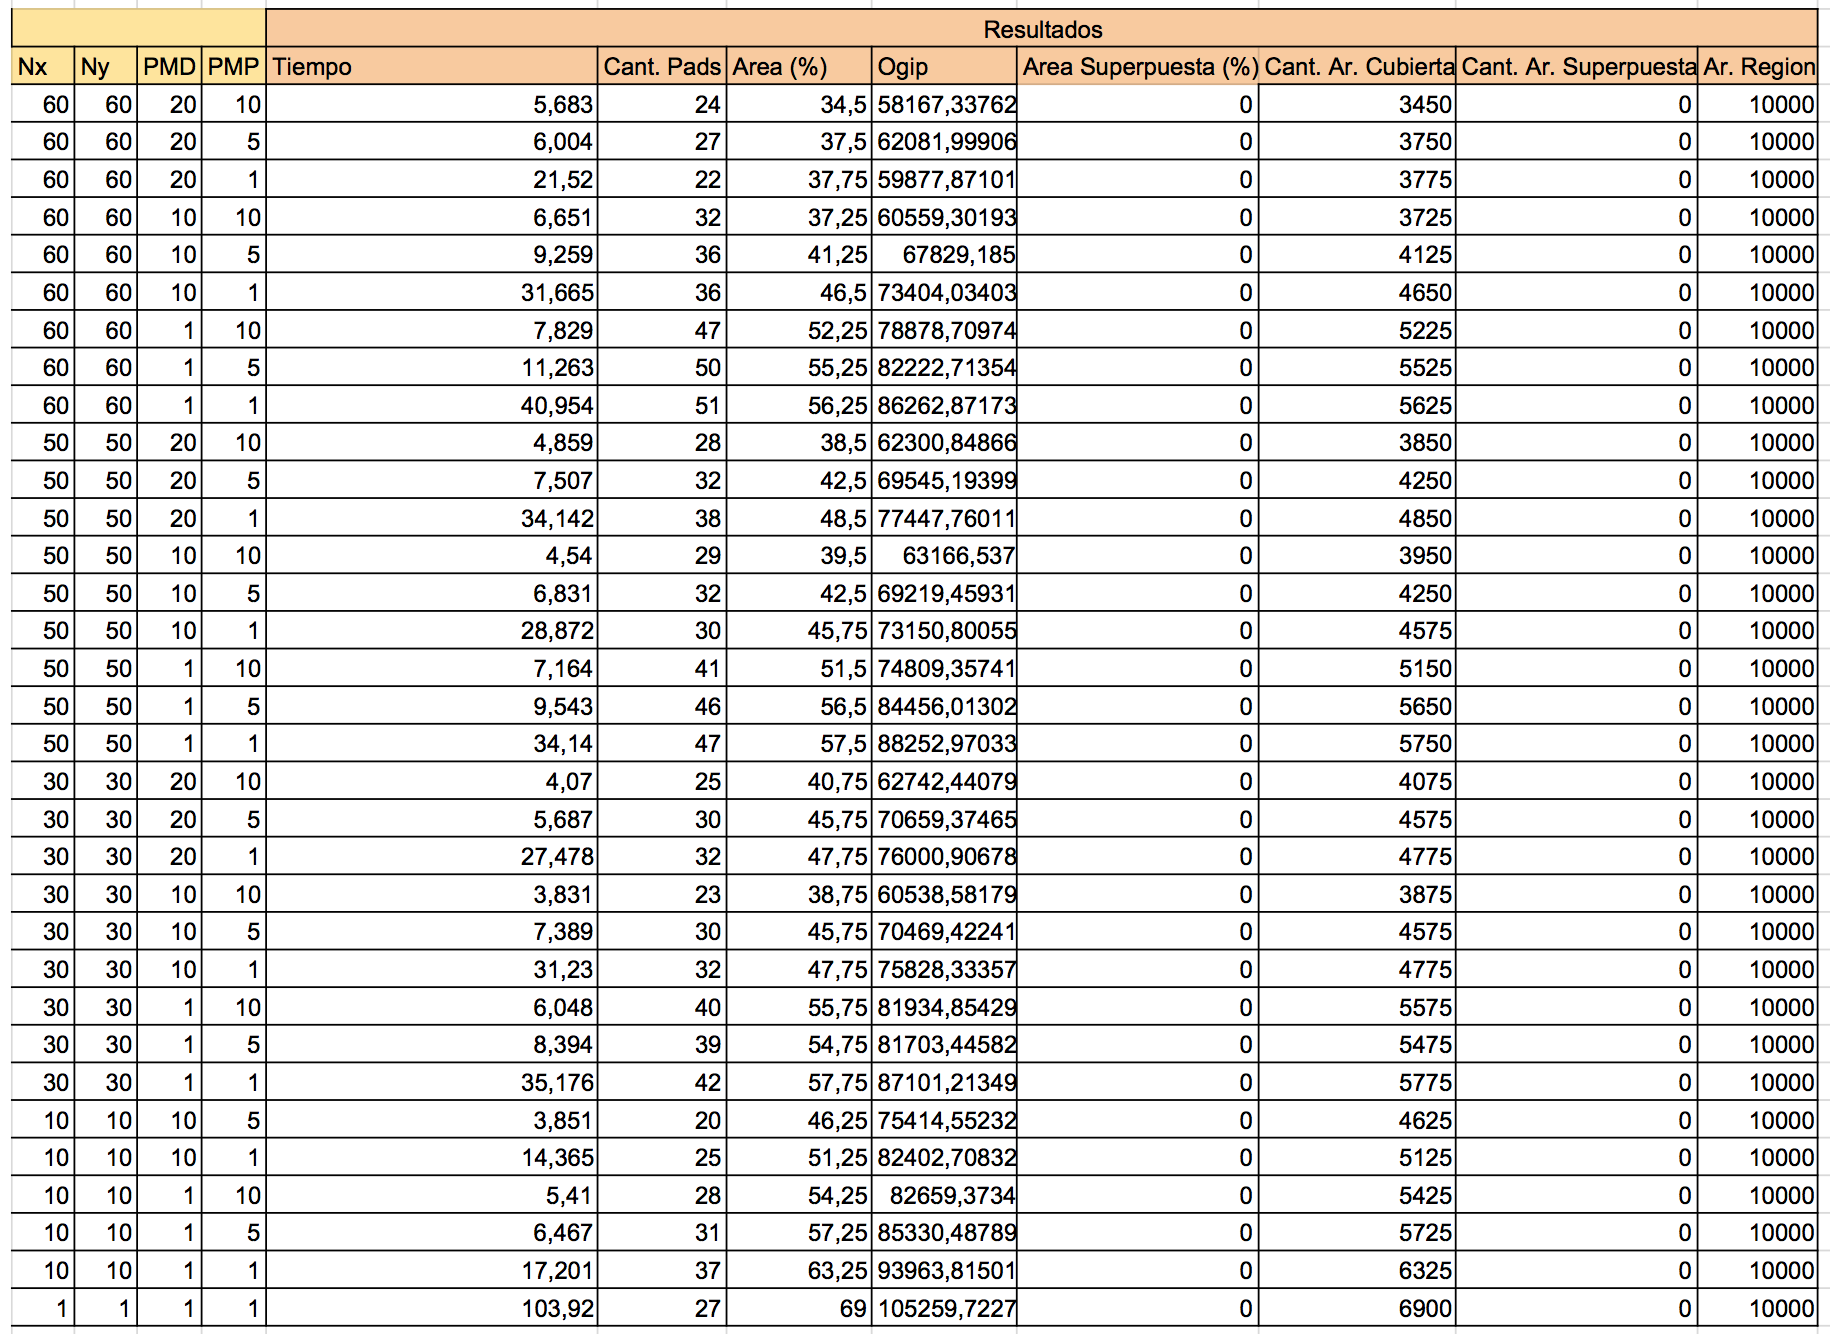
\includegraphics[width=1\textwidth]{imagenes/GML_45G100x100_muchos}
\end{center}

\begin{center}
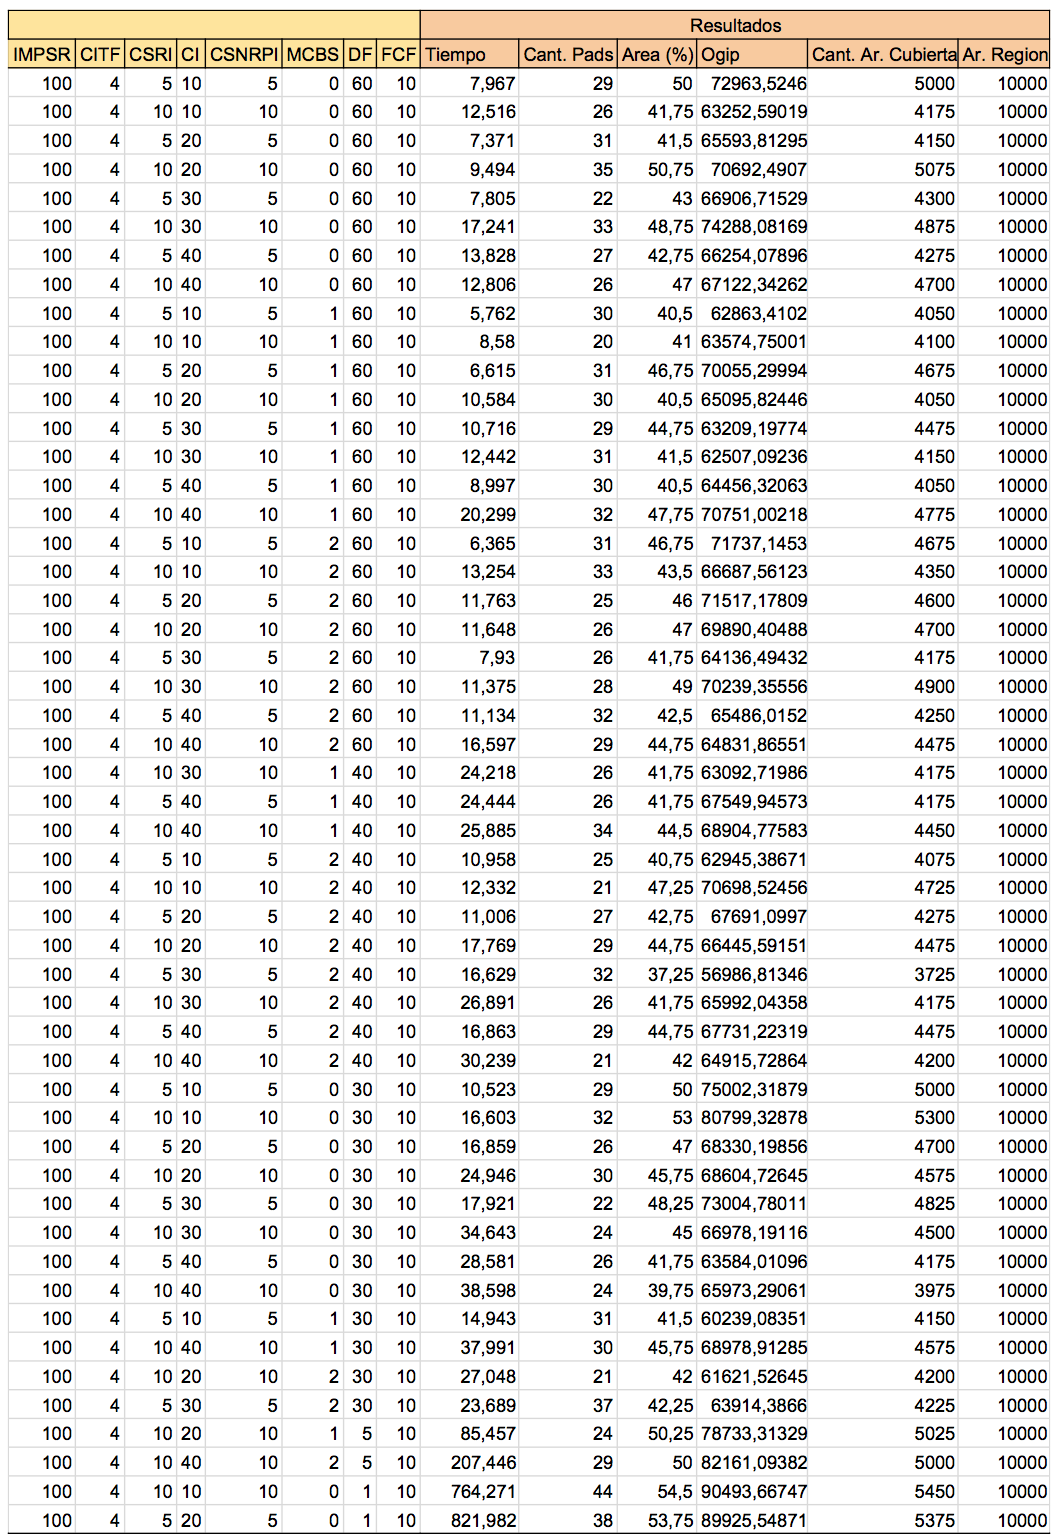
\includegraphics[width=1\textwidth]{imagenes/45G100x100_muchos_V1}
\end{center}

\begin{center}
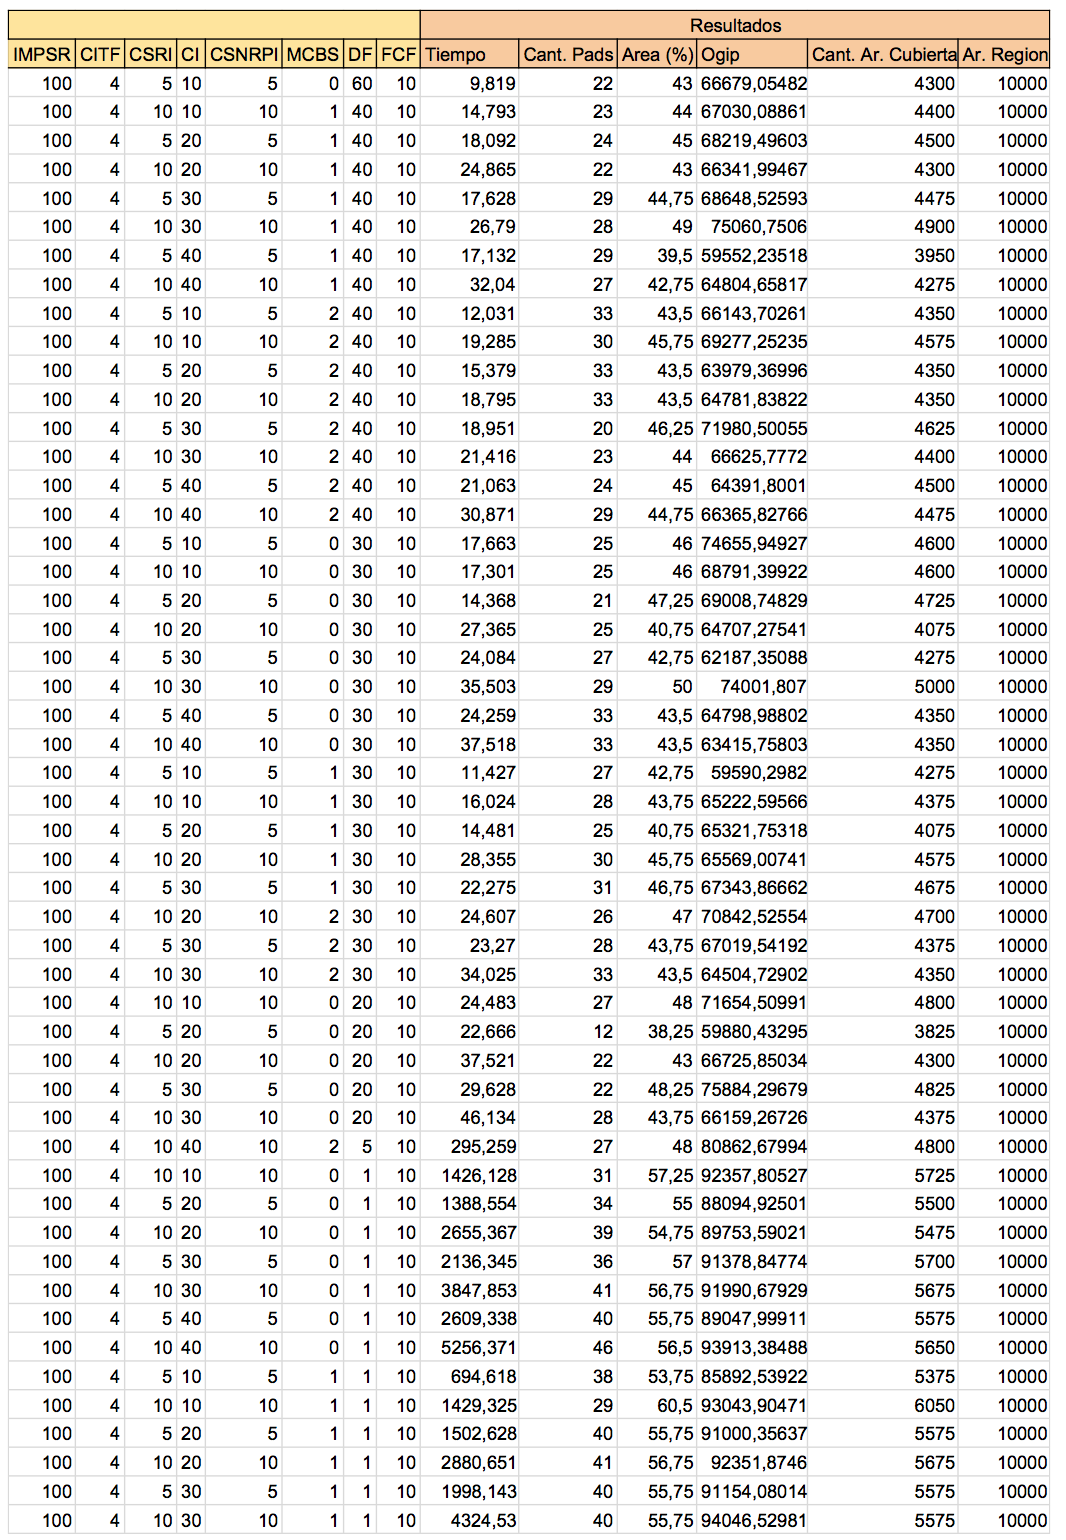
\includegraphics[width=1\textwidth]{imagenes/45G100x100_muchos_V2}
\end{center}

\subsection{inst2}

\begin{center}
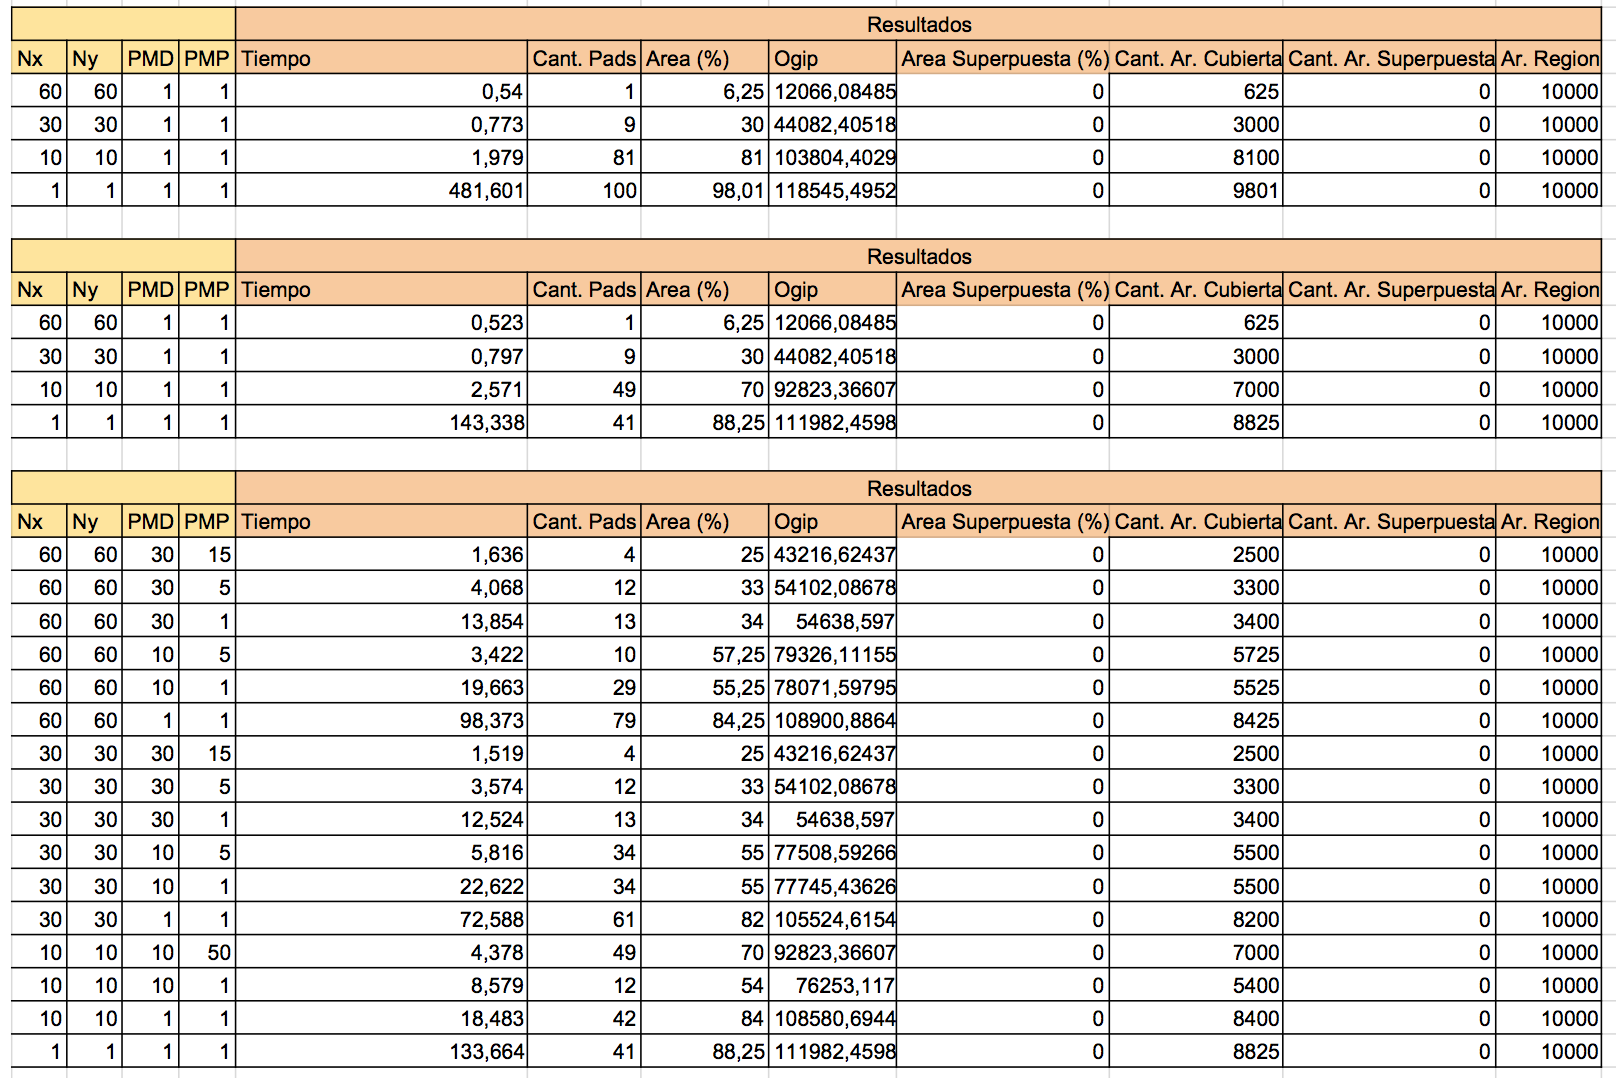
\includegraphics[width=1\textwidth]{imagenes/ALL_inst2}
\end{center}

\begin{center}
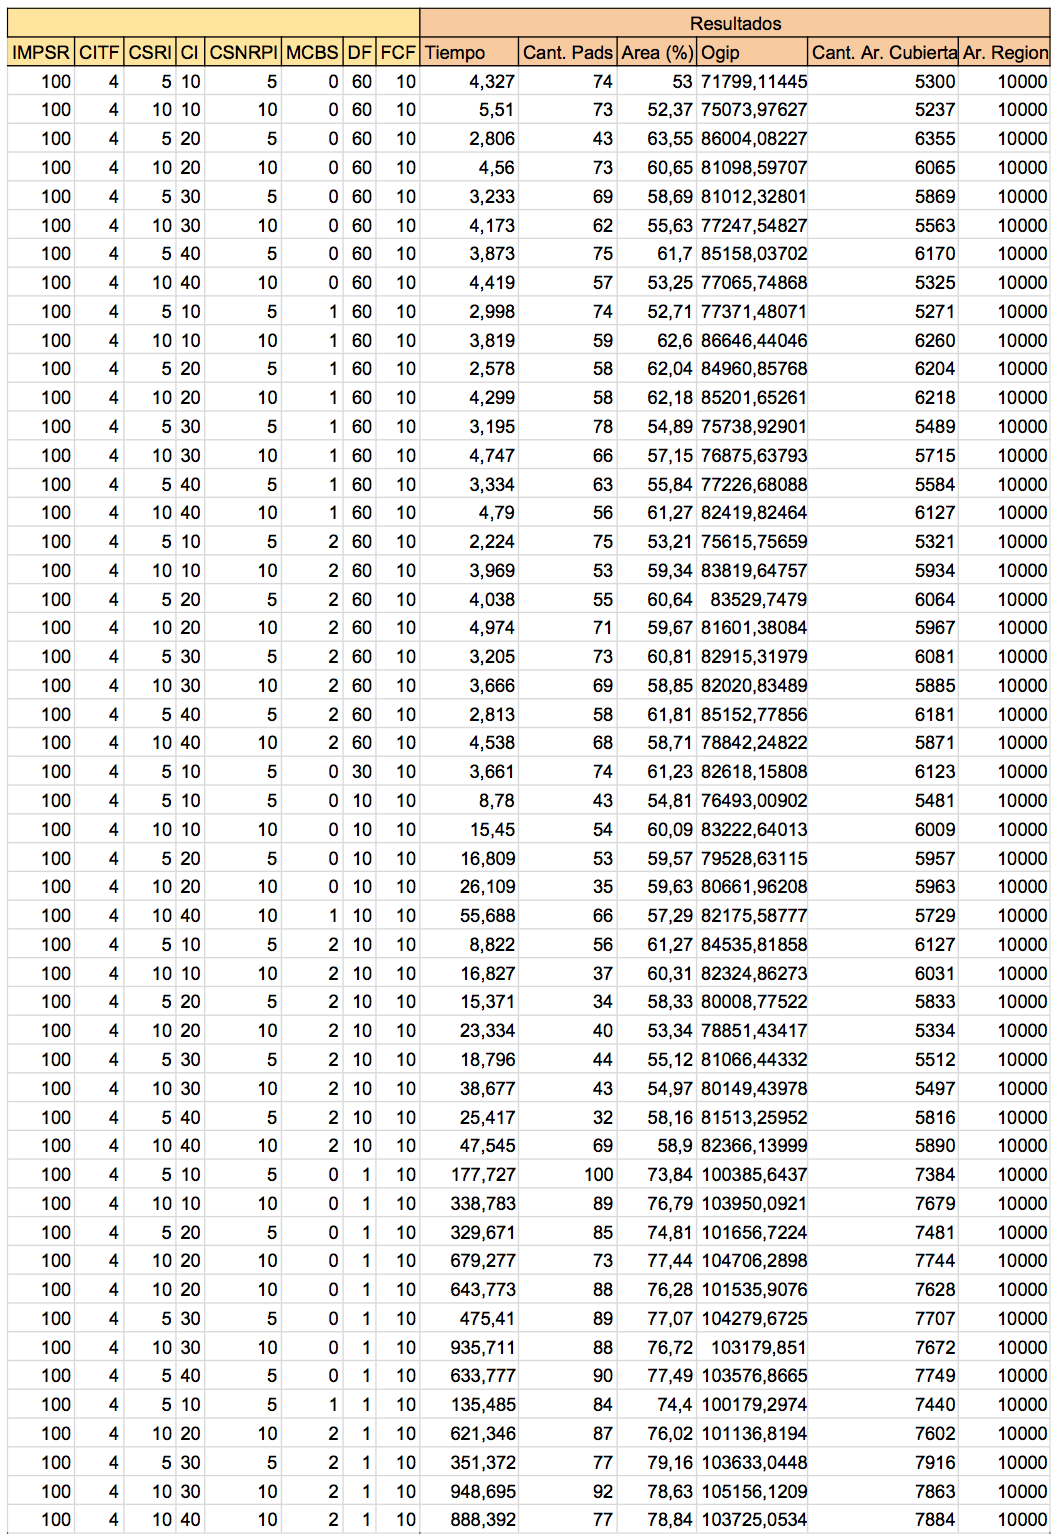
\includegraphics[width=1\textwidth]{imagenes/inst2_V1}
\end{center}

\begin{center}
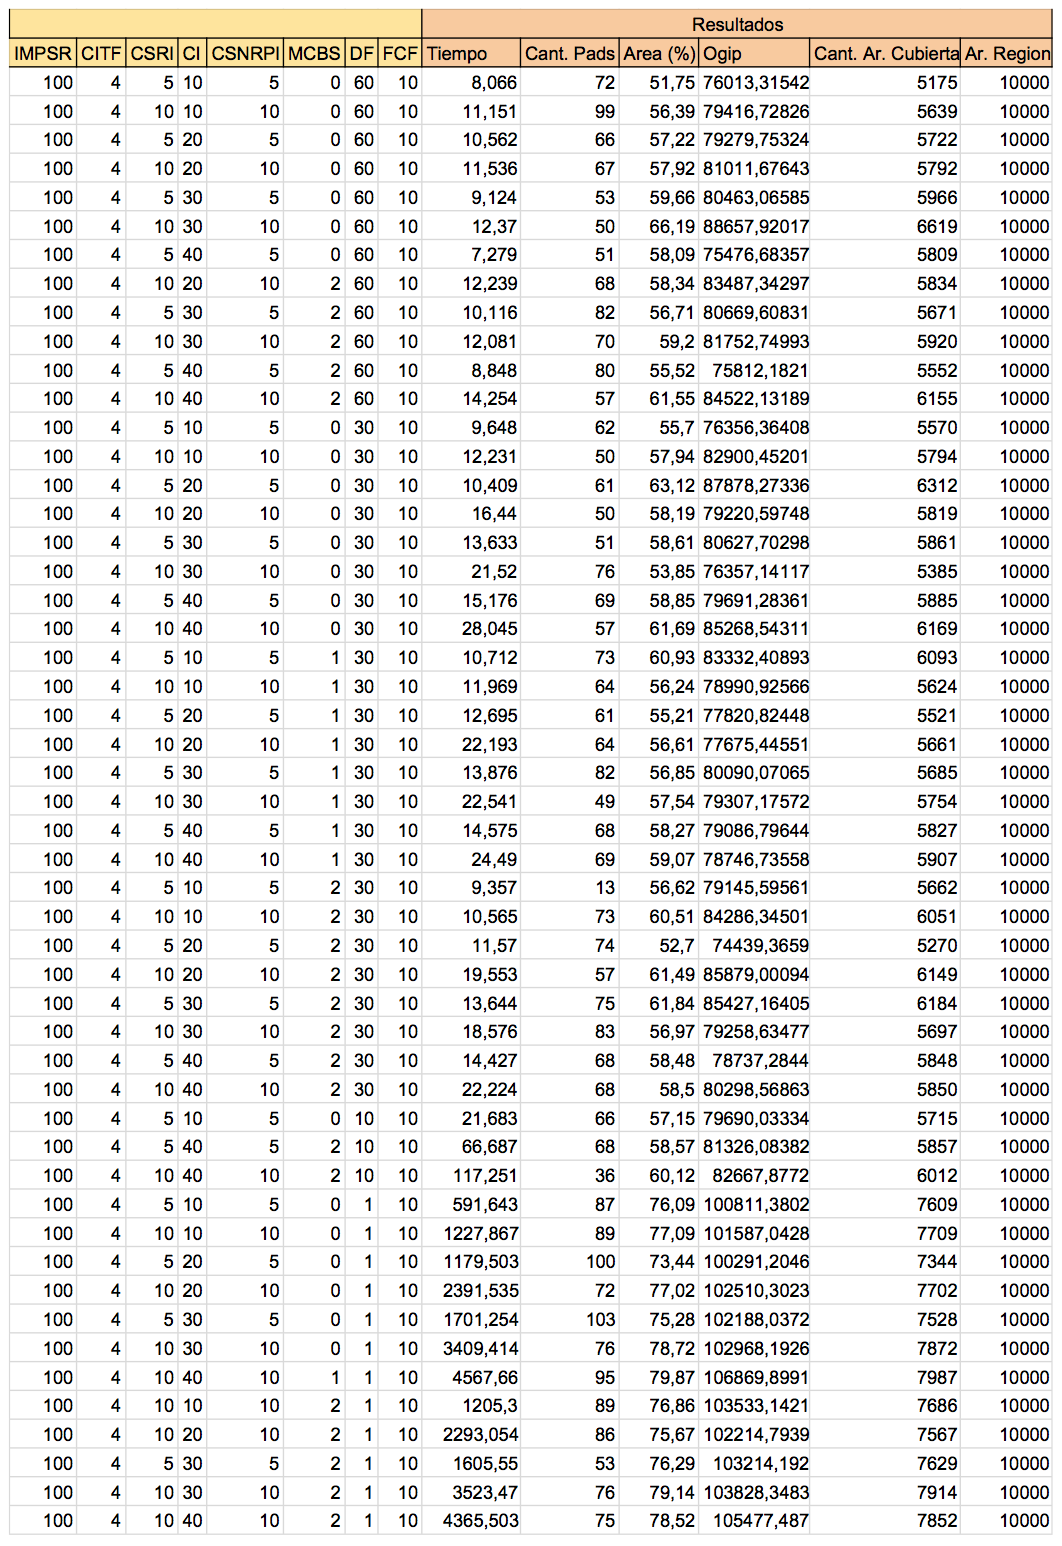
\includegraphics[width=1\textwidth]{imagenes/inst2_V2}
\end{center}

\subsection{45G110X90Y8E7AR}

\begin{center}
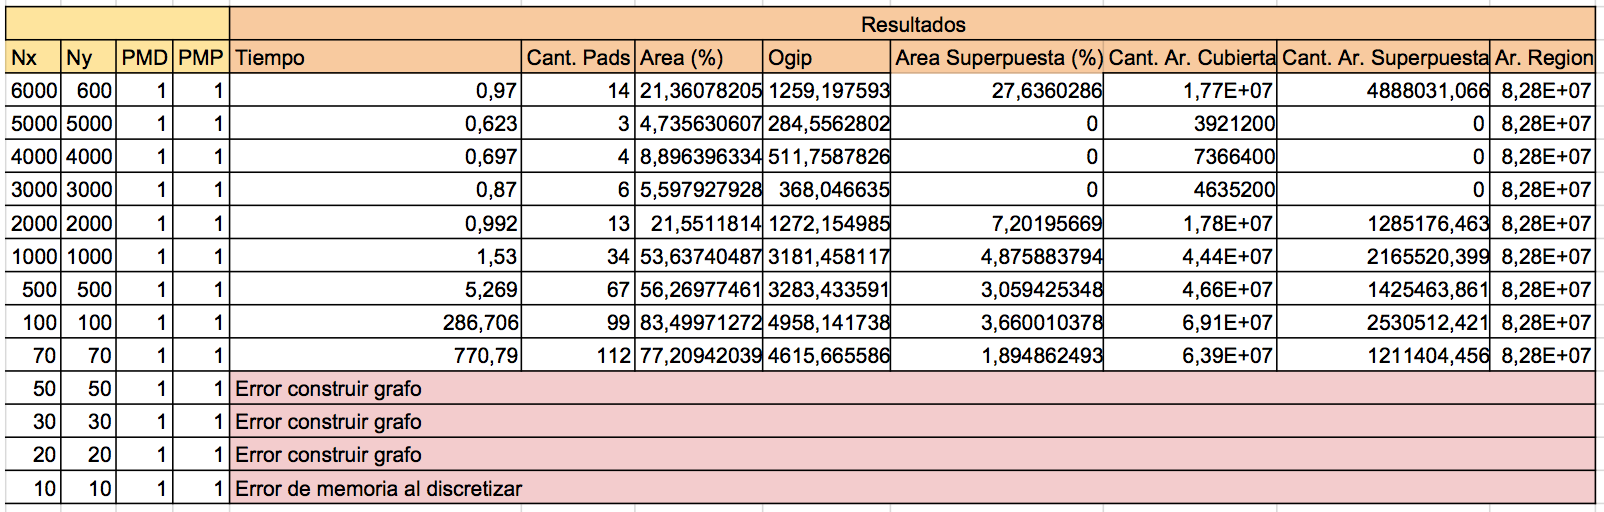
\includegraphics[width=1\textwidth]{imagenes/S_45G110X90Y8E7AR}
\end{center}

\begin{center}
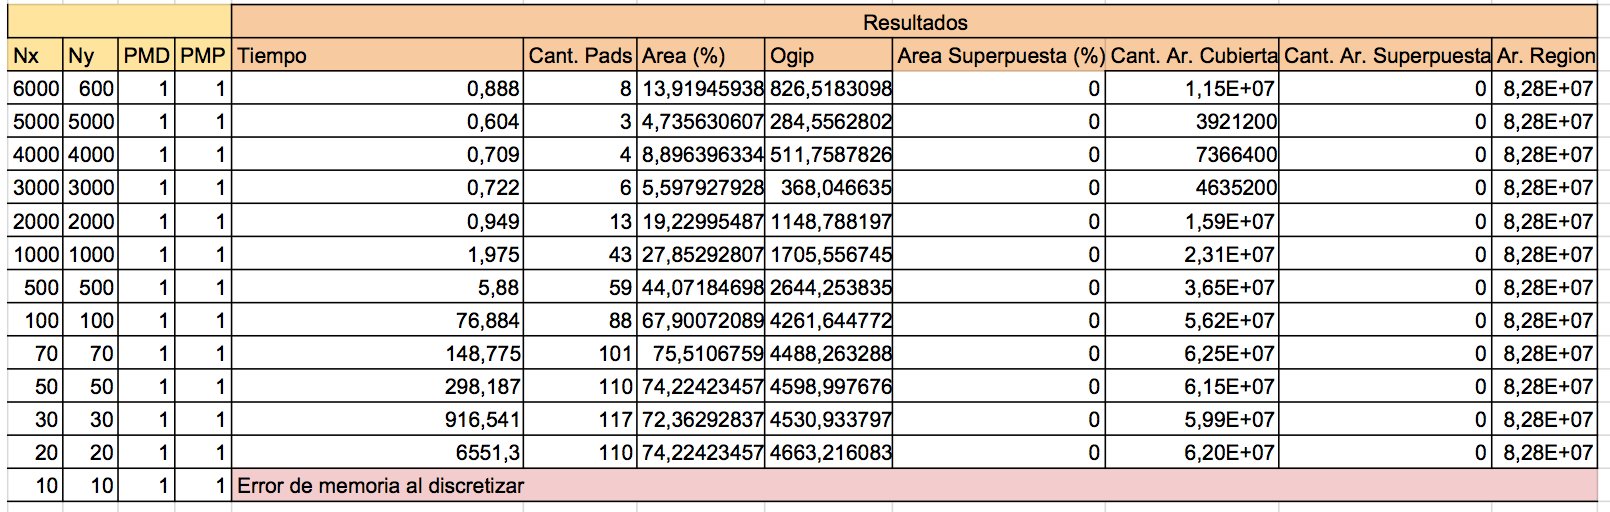
\includegraphics[width=1\textwidth]{imagenes/G_45G110X90Y8E7AR}
\end{center}

\begin{center}
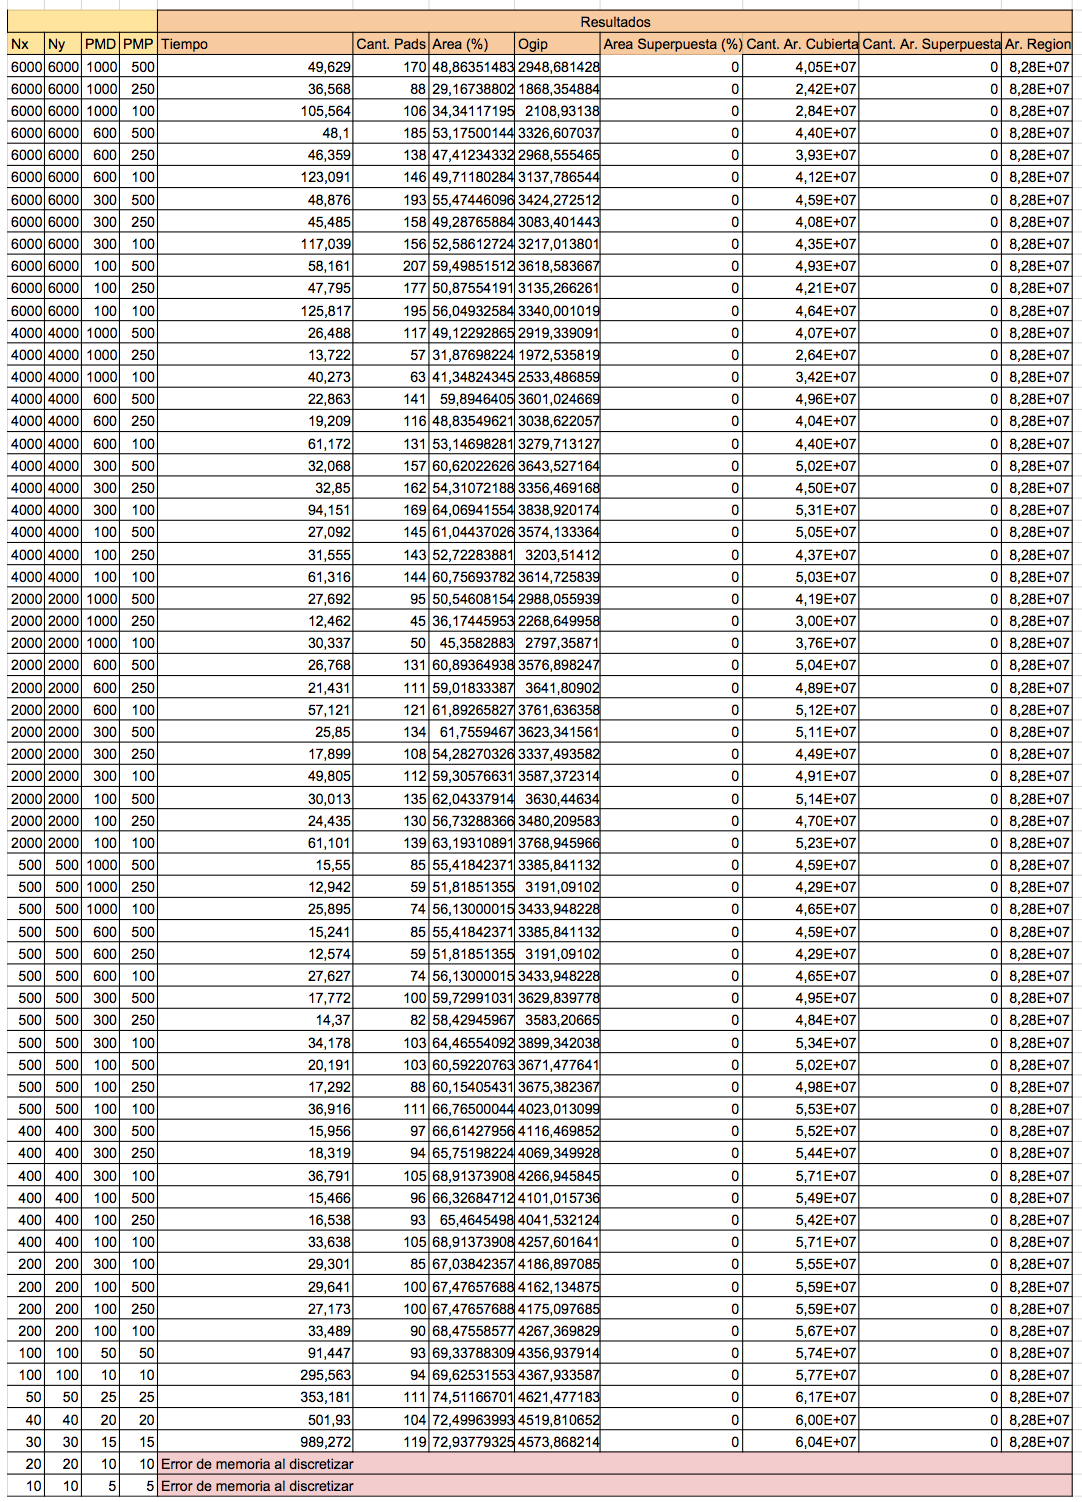
\includegraphics[width=1\textwidth]{imagenes/GML_45G110X90Y8E7AR}
\end{center}

\begin{center}
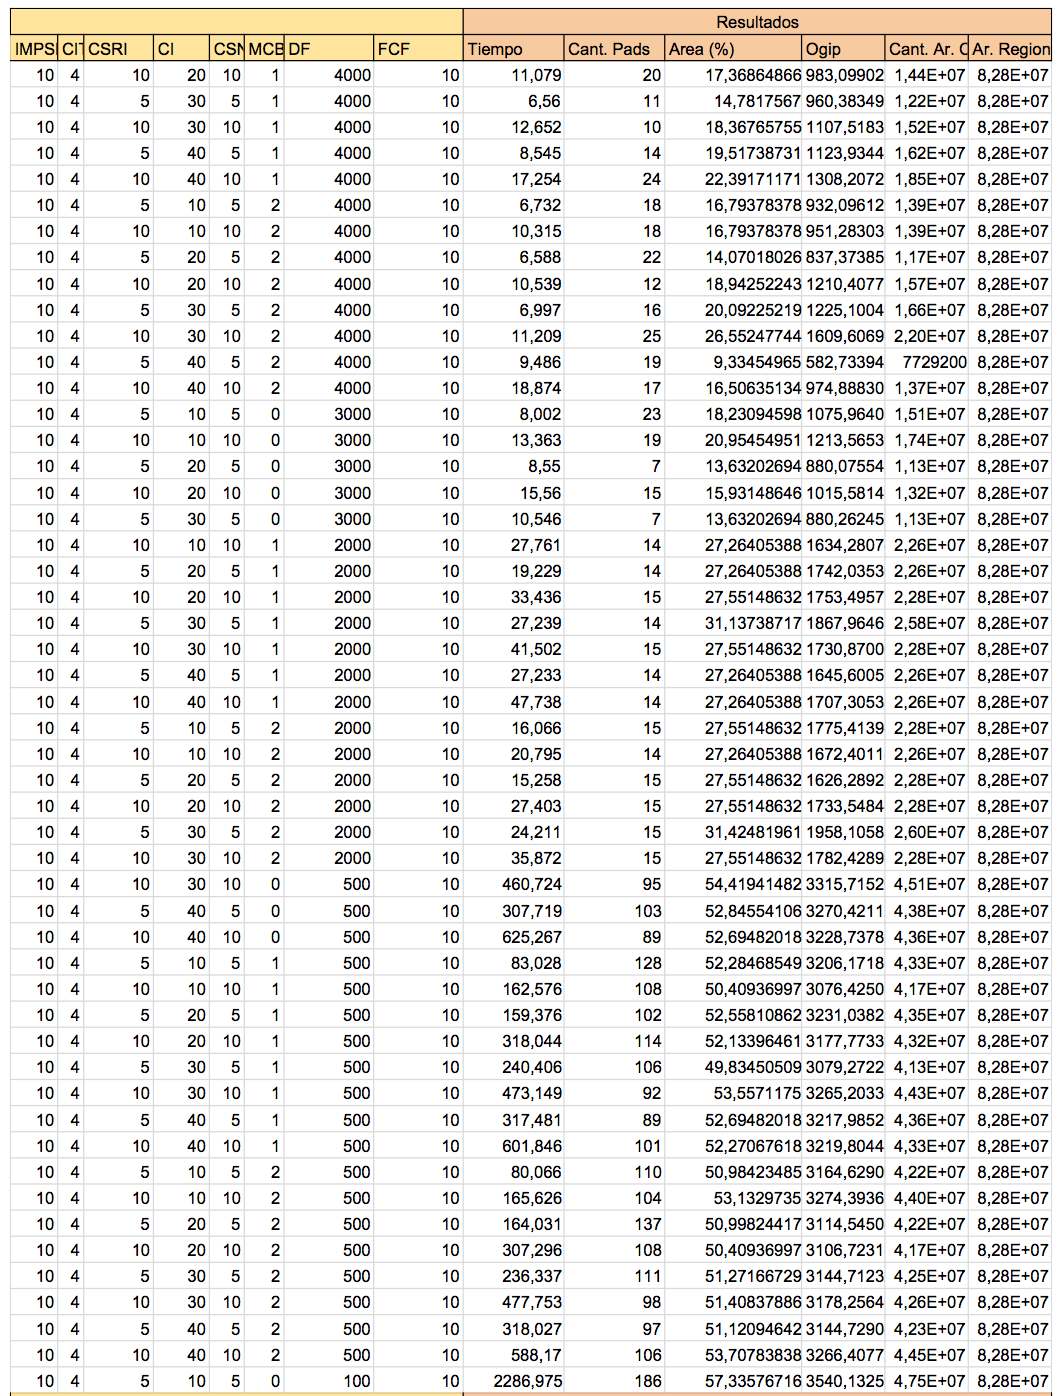
\includegraphics[width=1\textwidth]{imagenes/45G110X90Y8E7AR_V1}
\end{center}

\begin{center}
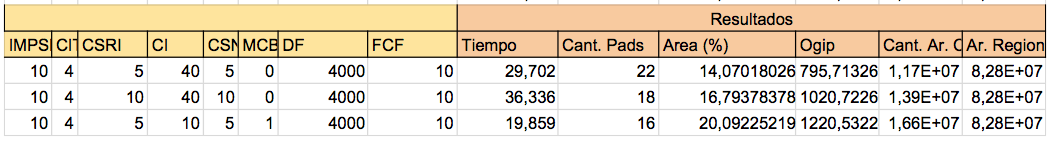
\includegraphics[width=1\textwidth]{imagenes/45G110X90Y8E7AR_V2_1}
\end{center}

\begin{center}
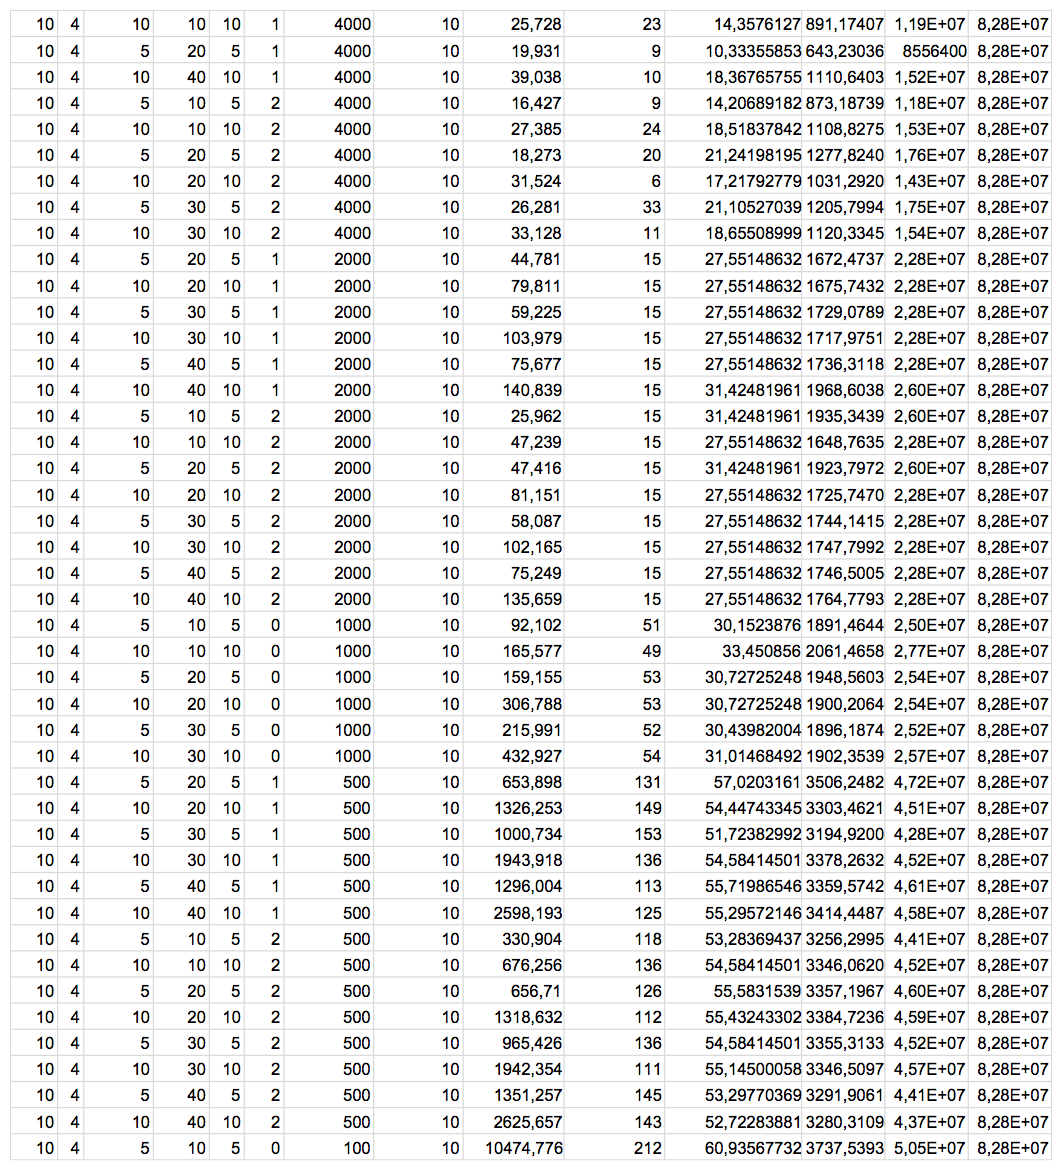
\includegraphics[width=1\textwidth]{imagenes/45G110X90Y8E7AR_V2_2}
\end{center}



\end{document}
